% =====================================================================
% Modeling Risk -- Problem Set 2 (2026)
% Full report linking theory, code (PS2/) and numerical results
% Compile with:  pdflatex -shell-escape main.tex   (twice for refs)
% =====================================================================
\documentclass[11pt,a4paper]{article}

% ---------- Encoding & language ----------
\usepackage[utf8]{inputenc}
\usepackage[T1]{fontenc}
\usepackage[english]{babel}
\usepackage{lmodern}
\usepackage{microtype}

% ---------- Math ----------
\usepackage{amsmath,amssymb,amsthm,mathtools}
\usepackage{bm}
\usepackage{dsfont}

% ---------- Layout ----------
\usepackage[a4paper,margin=2.4cm]{geometry}
\usepackage{setspace}
\usepackage{parskip}
\usepackage{booktabs}
\usepackage{array}
\usepackage{multirow}
\usepackage{multicol}
\usepackage{siunitx}
\sisetup{
  detect-all,
  group-separator={\,},
  output-decimal-marker={.}
}

% ---------- Floats ----------
\usepackage{graphicx}
\graphicspath{{../figures/}{./figures/}}
\usepackage{float}
\usepackage{caption}
\usepackage{subcaption}

% ---------- Refs & links ----------
\usepackage[colorlinks=true,
            linkcolor=blue!55!black,
            citecolor=blue!55!black,
            urlcolor=blue!55!black]{hyperref}
\usepackage{cleveref}

% ---------- Code listings ----------
\usepackage{xcolor}
\usepackage{listings}
\definecolor{codebg}{RGB}{248,248,248}
\definecolor{codekey}{RGB}{0,0,160}
\definecolor{codestr}{RGB}{160,40,40}
\definecolor{codecom}{RGB}{0,110,0}
\lstdefinestyle{py}{
  language=Python,
  basicstyle=\ttfamily\footnotesize,
  keywordstyle=\color{codekey}\bfseries,
  stringstyle=\color{codestr},
  commentstyle=\color{codecom}\itshape,
  showstringspaces=false,
  backgroundcolor=\color{codebg},
  frame=single,
  rulecolor=\color{black!25},
  framesep=4pt,
  framerule=0.4pt,
  breaklines=true,
  numbers=left,
  numberstyle=\tiny\color{black!50},
  numbersep=6pt,
  xleftmargin=2.2em,
}
\lstset{style=py}

% ---------- Theorem-like ----------
\newtheorem{prop}{Proposition}
\newtheorem{remark}{Remark}
\newtheorem{defn}{Definition}

% ---------- Macros ----------
\newcommand{\R}{\mathbb{R}}
\newcommand{\E}{\mathbb{E}}
\newcommand{\Var}{\operatorname{Var}}
\newcommand{\Cov}{\operatorname{Cov}}
\newcommand{\Cor}{\operatorname{Corr}}
\newcommand{\diag}{\operatorname{diag}}
\newcommand{\sgn}{\operatorname{sgn}}
\newcommand{\indic}{\mathds{1}}
\newcommand{\given}{\,|\,}
\newcommand{\Pphi}{\Phi}
\newcommand{\pphi}{\phi}
\DeclareMathOperator*{\argmax}{arg\,max}
\DeclareMathOperator*{\argmin}{arg\,min}
\newcommand{\code}[1]{\texttt{\small #1}}
\newcommand{\file}[1]{\texttt{\small\textcolor{blue!55!black}{#1}}}

% ---------- Title ----------
\title{\bfseries Modeling Risk --- Homework 2026\\[2pt]}
\author{Pedro José Piqueras Martínez\\\small Master in Economics and Data Science}
\date{April 2026}

\begin{document}
\maketitle

\begin{abstract}
\noindent
This report develops the theoretical answer to the homework of
\emph{Modeling Risk}. Every mathematical derivation is cross-referenced to
the Python implementation under \file{PS2/}, so that each printed number and
figure can be regenerated by running the corresponding \code{main.py}.
\end{abstract}

\tableofcontents
\bigskip\hrule

% ---------------------------------------------------------------------
\section{Introduction and notation}\label{sec:intro}
% ---------------------------------------------------------------------
A \emph{copula} is the joint distribution function of a random vector with uniform
marginals. By Sklar's theorem any joint distribution $F$ with marginals $F_1,\ldots,F_n$
can be written
\begin{equation}\label{eq:sklar}
F(x_1,\ldots,x_n)=C\!\bigl(F_1(x_1),\ldots,F_n(x_n)\bigr),
\end{equation}
Sklar's theorem is the central tool of the work: it allows us to model the
dependence structure (the copula $C$) separately from the univariate behaviour
of each return ($F_i$). The conditional CDF of the copula
\begin{equation}\label{eq:cond-cdf}
C(u_1\given u_2)=\frac{\partial}{\partial u_2}C(u_1,u_2)
\end{equation}
is the building block of all the simulation algorithms used below: drawing
$V_1,V_2$ i.i.d. uniform on $(0,1)$ and inverting $V_1=C(U_1\given V_2)$ in
$U_1$ produces a sample with the desired copula. We adopt the notation
$\Phi$ for the standard Normal CDF, $\phi$ for its density, $t_\nu$ for the
Student-$t$ CDF with $\nu$ degrees of freedom, and $\eta_t=\Phi^{-1}(u_t)$
for the Normal transform of a uniform.

\paragraph{Project layout.}
The whole numerical work is implemented in a single Python project
\file{PS2/} organised by exercise:
\begin{center}
\small
\begin{tabular}{ll}
\toprule
Folder & Content\\
\midrule
\file{exercise1/} & Bivariate simulation, portfolio statistics, IFM/CML estimation\\
\file{exercise2/} & GARCH/GJR + DCC on BTC/ETH/ADA returns\\
\file{exercise3/} & NM-copula conditional CDF and $q$-quantile inversion\\
\file{exercise4/} & Black--Scholes pricing + option-based portfolio simulation\\
\file{exercise5/} & Clayton DGP, copula MLE, Kupiec backtest\\
\file{config.json} & All numerical parameters consumed by every \code{main.py}\\
\file{figures/} & Generated figures and saved tables\\
\file{report/} & This LaTeX document\\
\bottomrule
\end{tabular}
\end{center}

\paragraph{Reproducibility.}
The file \code{main.py} runs all excercises and the report. 
However, each exercise can be launched from its own \code{main.py}. Each code loads the global
\file{config.json} and writes its outputs to \file{figures/}.
Random seeds are fixed in the configuration file. The exact tables and figures
shown below were obtained by running, from \file{PS2/},
\begin{lstlisting}[language=bash,numbers=none]
# for all excercises
python -m main
# for individual excercises
python -m exercise1.main
python -m exercise2.main
python -m exercise3.main
python -m exercise4.main
python -m exercise5.main
\end{lstlisting}

% ---------------------------------------------------------------------
% =====================================================================
\section{Exercise 1 -- Bivariate copula simulation, dependence, and IFM/CML}
\label{sec:ex1}
% =====================================================================

We work with six bivariate copulas (\textsc{Clayton} $\theta=10$, \textsc{Survival
Clayton} $\theta=5$, \textsc{Gaussian} $\rho=-0.7$, \textsc{Student-$t$}
$\rho=-0.7,\nu=5$, \textsc{FGM} $\lambda=-0.5$ and \textsc{FGM} $\lambda=0$).
The implementation lives in \file{exercise1/} and is driven by
\file{exercise1/main.py}. Throughout, $V_1,V_2$ denote independent
$\mathcal{U}(0,1)$ draws, while $(U_1,U_2)$
is the resulting copula sample.

% ---------------------------------------------------------------
\subsection{Theoretical building block: the conditional distribution method}
% ---------------------------------------------------------------

Given a bivariate copula $C$, define the partial derivative
\[
C_2(u_1\given u_2)\;=\;\Pr(U_1\le u_1\mid U_2=u_2)\;=\;\frac{\partial}{\partial u_2}\,C(u_1,u_2).
\]
By construction $C_2(\cdot\given u_2)$ is a CDF on $(0,1)$. The
\emph{conditional inversion algorithm} produces a sample from $C$ in two steps:
\[
\boxed{\;U_2\sim\mathcal{U}(0,1),\qquad U_1\;=\;C_2^{-1}(V_1\given U_2),\quad V_1\sim\mathcal{U}(0,1).\;}
\]
This is what every routine in \file{exercise1/copula\_sim.py} implements.

% ---------------------------------------------------------------
\subsection{Closed-form simulators}
% ---------------------------------------------------------------

\paragraph{Clayton ($\theta>0$).}
$C^{Cla}(u_1,u_2)=\bigl(u_1^{-\theta}+u_2^{-\theta}-1\bigr)^{-1/\theta}$.
Differentiating in $u_2$,
\[
C_2(u_1\given u_2)=u_2^{-\theta-1}\bigl(u_1^{-\theta}+u_2^{-\theta}-1\bigr)^{-1-1/\theta}.
\]
Setting $C_2=v_1$ and solving for $u_1$ yields
\begin{equation}\label{eq:clayton-sim}
U_1=\Bigl[\,1+u_2^{-\theta}\bigl(v_1^{-\theta/(\theta+1)}-1\bigr)\Bigr]^{-1/\theta}.
\end{equation}

\paragraph{Survival Clayton.} The survival copula
$\hat C(u_1,u_2)=u_1+u_2-1+C(1-u_1,1-u_2)$ is sampled by drawing
$(\tilde U_1,\tilde U_2)$ from Clayton and setting
$U_i=1-\tilde U_i$, which produces the upper-tail counterpart of the Clayton.

\paragraph{Gaussian ($-1<\rho<1$).}
With $X_i=\Phi^{-1}(U_i)$,
\[
X_1\given X_2=x_2\;\sim\;\mathcal{N}\!\bigl(\rho x_2,\;1-\rho^2\bigr),
\]
so the conditional CDF is $C^G(u_1\given u_2)=
\Phi\!\bigl((\Phi^{-1}u_1-\rho\,\Phi^{-1}u_2)/\sqrt{1-\rho^2}\bigr)$
and the inverse gives
\begin{equation}\label{eq:gauss-sim}
U_1=\Phi\!\bigl(\rho\,\Phi^{-1}(u_2)+\sqrt{1-\rho^2}\,\Phi^{-1}(v_1)\bigr).
\end{equation}

\paragraph{Student $t$ ($\rho,\nu$).} Letting $y_i=t_\nu^{-1}(u_i)$,
\[
\frac{\,Y_1-\rho Y_2\,}{\sqrt{(1-\rho^2)(\nu+Y_2^2)/(\nu+1)}}\;\sim\;t_{\nu+1},
\]
which inverts to
\begin{equation}\label{eq:t-sim}
U_1=t_\nu\!\Bigl(\rho\, Y_2+t_{\nu+1}^{-1}(v_1)\sqrt{(1-\rho^2)(\nu+Y_2^2)/(\nu+1)}\Bigr).
\end{equation}

\paragraph{FGM ($-1\le\lambda\le 1$).}
$C^{FGM}(u_1,u_2)=u_1u_2[1+\lambda(1-u_1)(1-u_2)]$. Setting
$\psi=\lambda(1-2u_2)$, the equation $C_2(u_1\given u_2)=v_1$ becomes
$\psi u_1^2-(1+\psi)u_1+v_1=0$, with the admissible root
\begin{equation}\label{eq:fgm-sim}
U_1=\frac{(1+\psi)-\sqrt{(1+\psi)^2-4\psi v_1}}{2\psi}\,.
\end{equation}
At $\lambda=0$ we have independence and $U_1=v_1$ is recovered as the limit.

\paragraph{Mixture (used in 1.d).} A copula mixture
$C=\pi C_A+(1-\pi)C_B$ is sampled by drawing a Bernoulli($\pi$) indicator
and selecting $C_A$ or $C_B$.

% ---------------------------------------------------------------
\subsection{1.a -- Scatter plots and dependence measures}
% ---------------------------------------------------------------

For each copula we draw $N=10^5$ pairs and compute the three
dependence measures: Pearson's $\rho$, Spearman's $\rho_S$ and Kendall's $\tau$.
Pearson is sensitive to the marginals and an average, while Spearman and Kendall 
capture better tail dependence.
Numerical results (Table~\ref{tab:1a}) and scatter plots
(Figure~\ref{fig:1a}) show:
\begin{itemize}\setlength\itemsep{0pt}
\item Clayton has lower-tail dependence.
\item Survival Clayton has upper-tail dependence.
\item Gaussian and Student-$t$ at $\rho=-0.7$ produce the elliptical dependence;
      $t$ adds heavier joint extremes.
\item FGM is essentially close to independence: its dependence parameter
      is bounded ($|\tau|\le 2/9$).
\end{itemize}

\begin{table}[H]\centering\small
\caption{Dependence measures, $N=10^5$ draws.}\label{tab:1a}
\begin{tabular}{lrrr}
\toprule
Copula & Pearson & Spearman & Kendall\\\midrule
Clayton $\theta=10$            & $0.9584$ & $0.9583$ & $0.8335$\\
Survival Clayton $\theta=5$    & $0.8844$ & $0.8847$ & $0.7141$\\
Gaussian $\rho=-0.7$           & $-0.6840$ & $-0.6839$ & $-0.4947$\\
Student-$t$ $\rho=-0.7,\nu=5$  & $-0.6723$ & $-0.6722$ & $-0.4948$\\
FGM $\lambda=-0.5$             & $-0.1706$ & $-0.1706$ & $-0.1139$\\
FGM $\lambda=0$                & $-0.0044$ & $-0.0044$ & $-0.0029$\\
\bottomrule
\end{tabular}
\end{table}

\begin{figure}[H]\centering
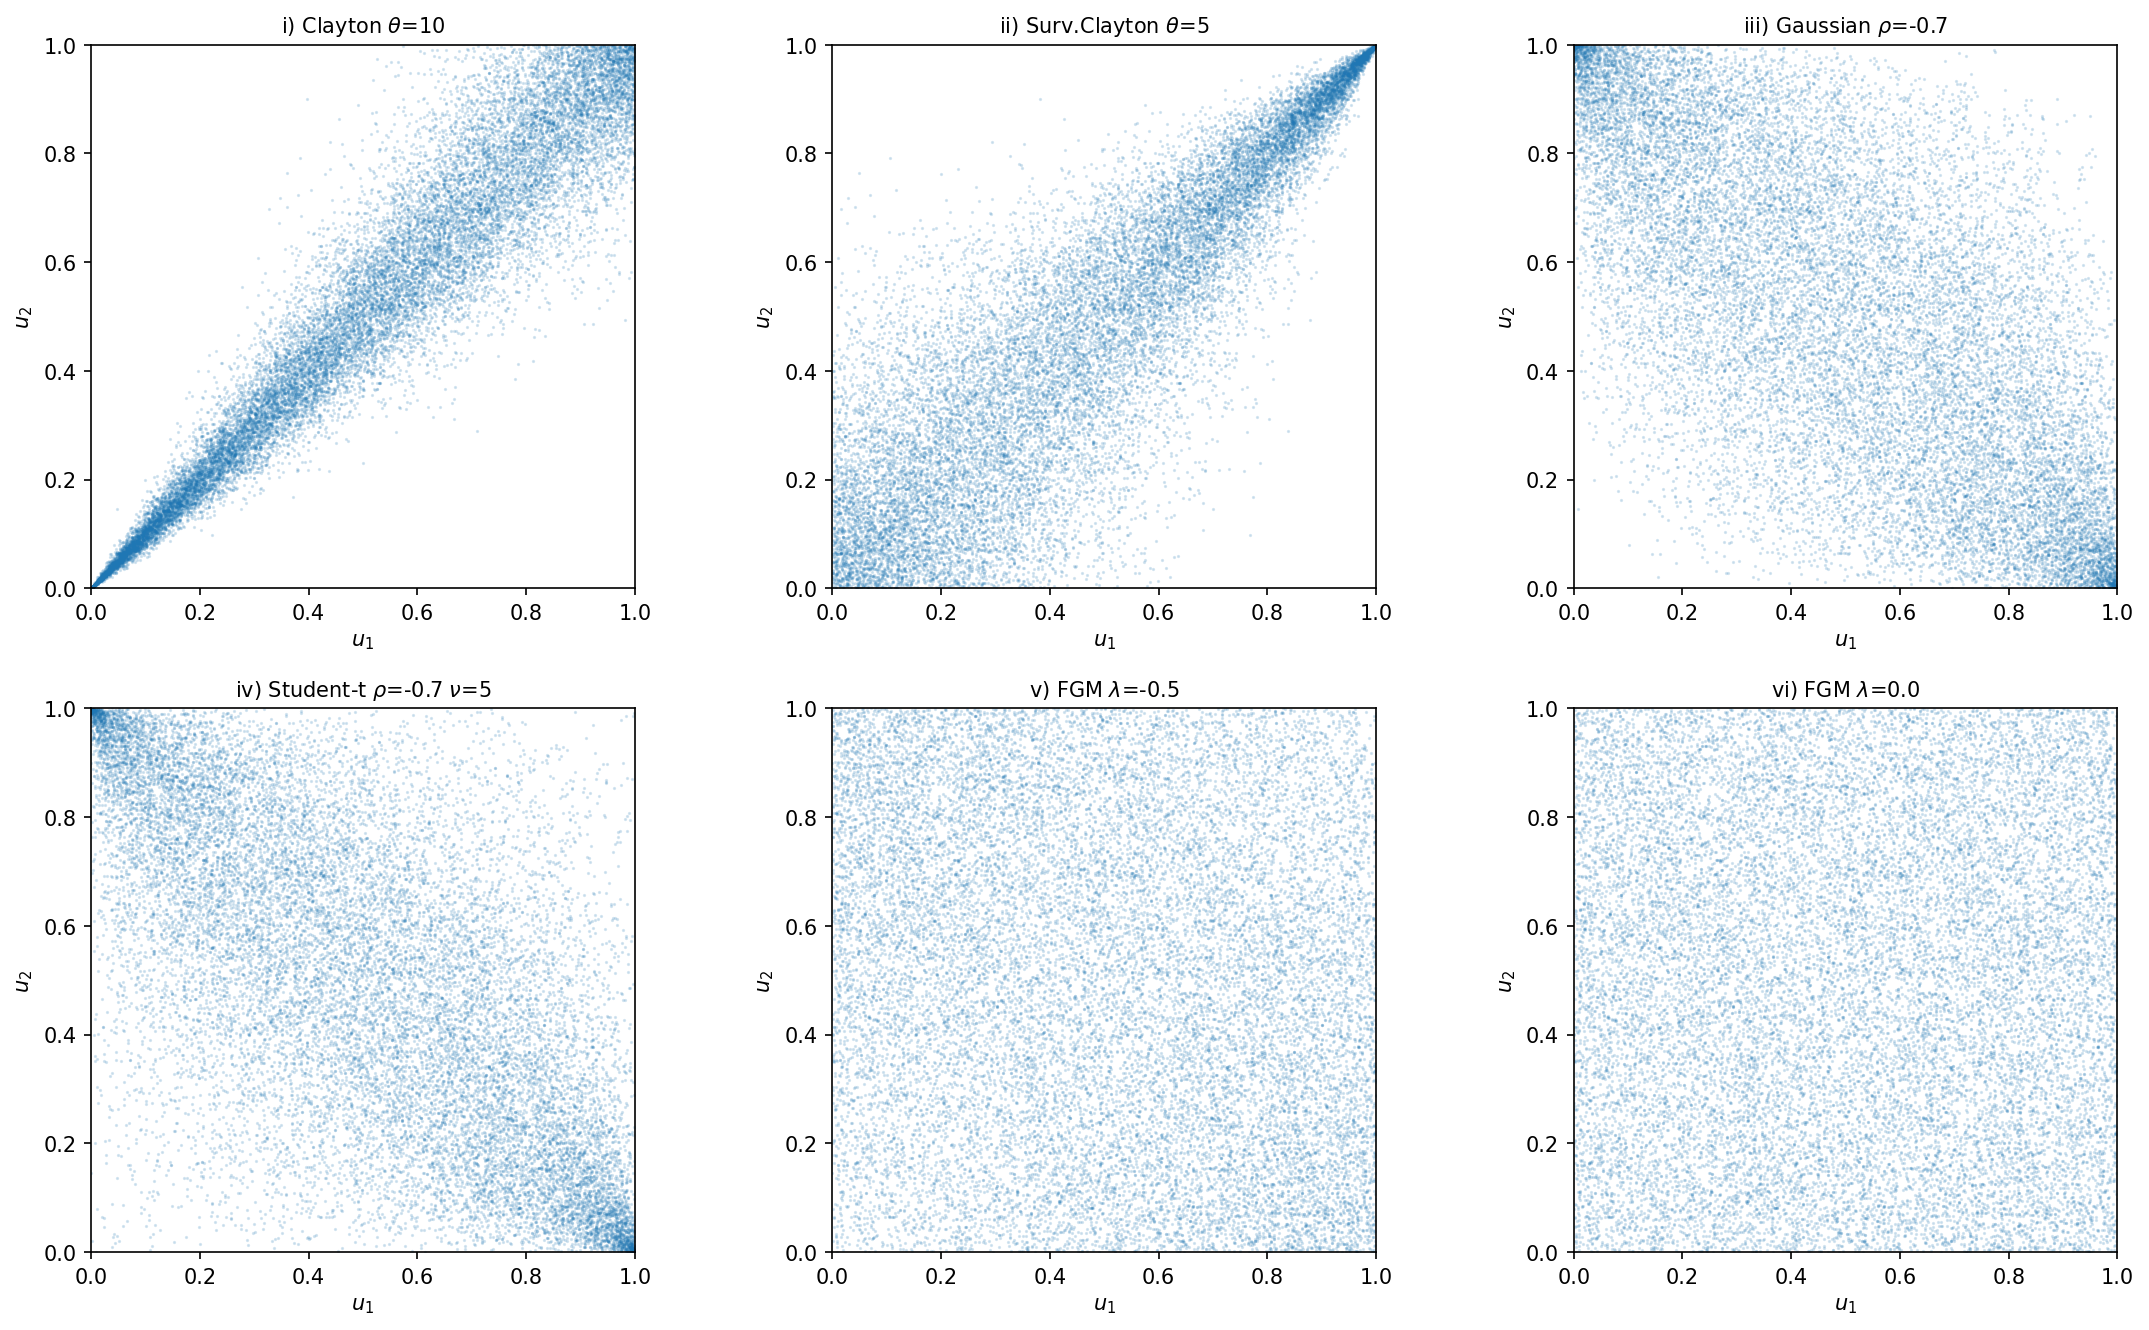
\includegraphics[width=0.95\linewidth]{fig_1a_scatter.png}
\caption{Dependent $\mathcal{U}(0,1)$ scatter plots, $N=10^5$.}\label{fig:1a}
\end{figure}

\paragraph{Kendall's $\tau$:} For Clayton,
$\tau=\theta/(\theta+2)=10/12=0.8333$, matching the simulated $0.8335$. For
Gaussian/$t$, $\tau=(2/\pi)\arcsin\rho=-0.4936$, matching $-0.4947$ and $-0.4948$.

% ---------------------------------------------------------------
\subsection{1.b -- Portfolio statistics, VaR, and correlation across copulas}
% ---------------------------------------------------------------

We build the portfolio $r_p=0.4\,r_1+0.6\,r_2$ where
$r_1=\Phi^{-1}(U_1)\sim\mathcal{N}(0,1)$ and
$r_2=t_6^{-1}(U_2)\sim t_6$. The marginals enter only through their quantile
functions; the copula governs the joint behaviour. Statistics are reported
in Table~\ref{tab:1b}, and a direct comparison of histograms vs.\ a Normal
overlay (same $\mu,\sigma$) is shown in Figure~\ref{fig:1b}.

\begin{table}[H]\centering\small
\caption{Portfolio statistics for $r_p=0.4r_1+0.6r_2$, $r_1\!\sim\!\mathcal{N}(0,1)$,
$r_2\!\sim\!t_6$.}\label{tab:1b}
\begin{tabular}{lrrrrrr}
\toprule
Copula & Mean & Std & Skew & Kurt & VaR$_{1\%}$ & VaR$_{5\%}$\\\midrule
Clayton           & $0.0007$ & $1.1116$ & $-0.1683$ & $4.1135$ & $-2.7795$ & $-1.8168$\\
Surv. Clayton     & $0.0012$ & $1.0915$ & $\phantom{-}0.2290$ & $4.0641$ & $-2.4421$ & $-1.6886$\\
Gaussian          & $0.0007$ & $0.5394$ & $-0.0197$ & $6.6978$ & $-1.3527$ & $-0.8432$\\
Student-$t$       & $0.0008$ & $0.5399$ & $\phantom{-}0.0029$ & $6.8199$ & $-1.3815$ & $-0.8472$\\
FGM $\lambda=-0.5$ & $0.0010$ & $0.7786$ & $-0.0039$ & $5.1494$ & $-1.9349$ & $-1.2390$\\
FGM $\lambda=0$    & $0.0011$ & $0.8342$ & $-0.0023$ & $4.7379$ & $-2.0458$ & $-1.3340$\\
\bottomrule
\end{tabular}
\end{table}

\begin{figure}[H]\centering
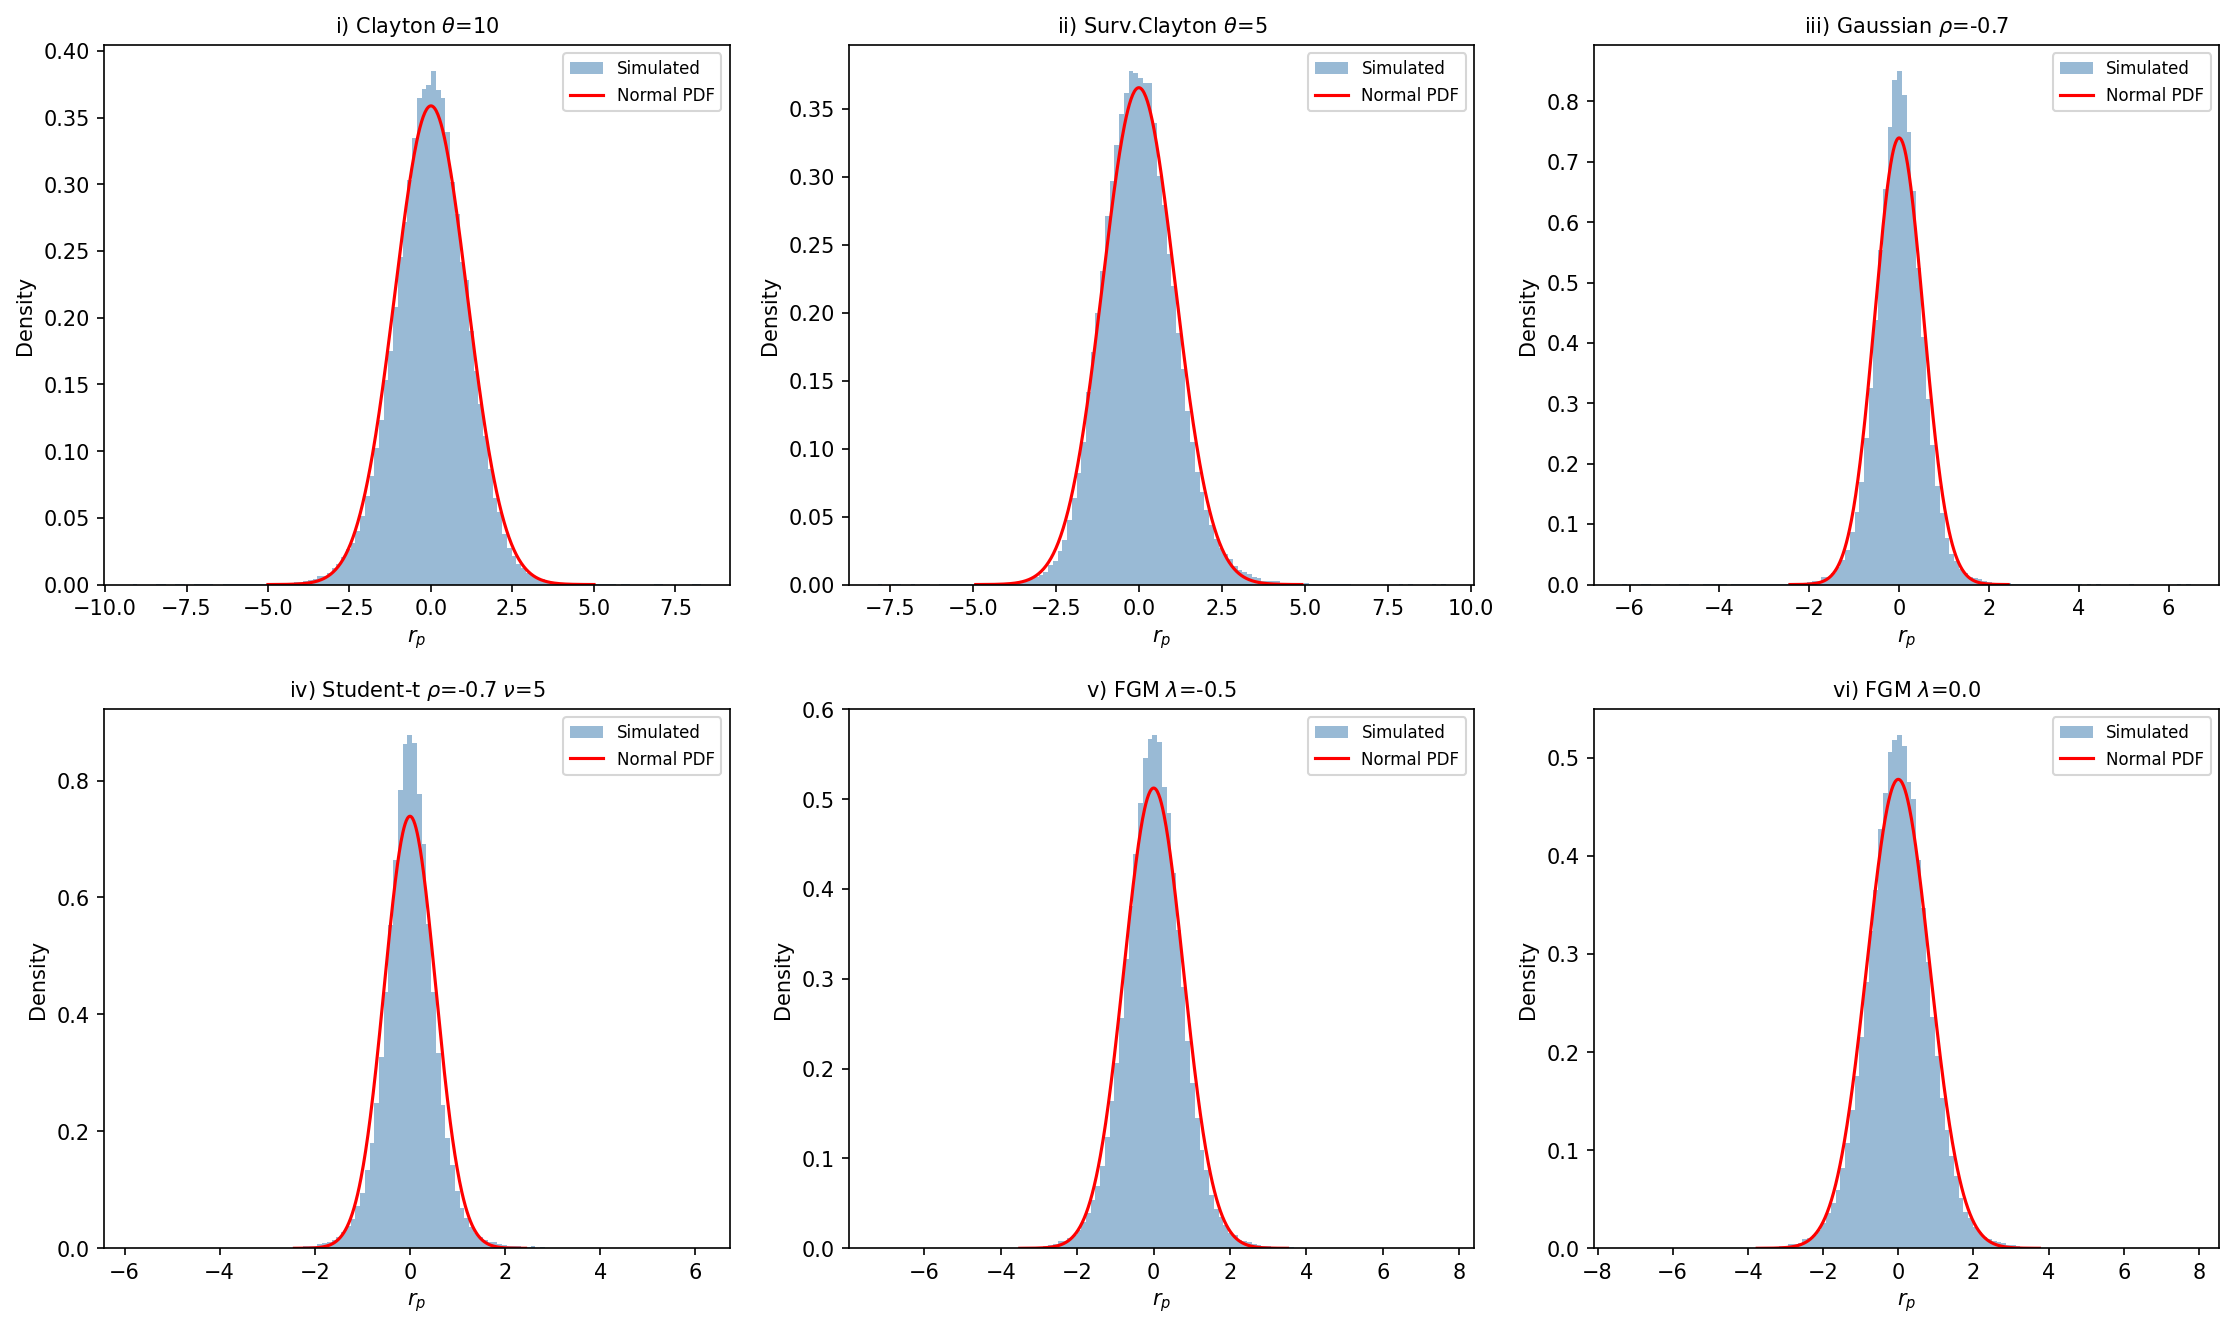
\includegraphics[width=0.95\linewidth]{fig_1b_histograms.png}
\caption{Portfolio return histograms with Normal($\mu,\sigma^2$) overlay.}\label{fig:1b}
\end{figure}

\paragraph{Reading the table.}
The variance of $r_p$ is
\[
\Var(r_p)=w_1^2\Var(r_1)+w_2^2\Var(r_2)+2w_1w_2\Cov(r_1,r_2),
\]
so a positive copula increases $\Var(r_p)$ relative to a negatively dependent
one (compare Clayton vs.\ Gaussian). VaR at level $\alpha$ is the empirical
$\alpha$-quantile $\widehat{\mathrm{VaR}}_\alpha=\hat F_{r_p}^{-1}(\alpha)$
Negative dependence (Gaussian $\rho=-0.7$) drastically reduces $\sigma_p$ and
hence the magnitude of VaR, as expected from diversification.

\newpage
% ---------------------------------------------------------------
\subsection{1.c -- Estimating a Gaussian copula by IFM with EDF margins}
% ---------------------------------------------------------------

Given an i.i.d. sample $\{(r_{1t},r_{2t})\}_{t=1}^T$ the Inference-Functions-for-Margins
(IFM) estimator proceeds in two steps:
\begin{enumerate}\setlength\itemsep{0pt}
\item Estimate each marginal $\hat F_i$ separately;
\item Estimate the copula parameter by maximising the copula log-likelihood
      evaluated at $\hat u_{it}=\hat F_i(r_{it})$.
\end{enumerate}
When $\hat F_i$ is the empirical CDF $\hat F_i(x)=\frac{1}{T+1}\sum_t \indic\{r_{it}\le x\}$
(``EDF'' margin) we obtain the \emph{Canonical Maximum Likelihood} (CML) variant.
The shift from $T$ to $T+1$ avoids values that would blow up
$\Phi^{-1}(\hat u)$.

\paragraph{Gaussian copula log-likelihood (slides eq.\,31).}
Let $\eta_t=(\Phi^{-1}\hat u_{1t},\Phi^{-1}\hat u_{2t})^\top$ and
$\Psi=\bigl(\begin{smallmatrix}1&\rho\\\rho&1\end{smallmatrix}\bigr)$. Then
\begin{align}
\ln c^G(\hat u_{1t},\hat u_{2t};\rho)
&=-\tfrac12\ln(1-\rho^2)
 -\tfrac12\,\eta_t^\top(\Psi^{-1}-I)\eta_t\notag\\
&=-\tfrac12\ln(1-\rho^2)-\frac{\rho^2(\eta_{1t}^2+\eta_{2t}^2)-2\rho\eta_{1t}\eta_{2t}}{2(1-\rho^2)}.
\label{eq:gauss-cop-ll}
\end{align}
We maximise $\sum_t \ln c^G$ in $\rho$ by Brent's method on $(-0.999,0.999)$
(\code{exercise1.estimation}).

\paragraph{Result.} On the Gaussian-copula sample with true $\rho=-0.7$ we obtain
$\hat\rho=-0.702095$, $\ln L=33{,}949.36$, with successful convergence. The
estimator recovers the truth to three decimals on $10^5$ observations.

% ---------------------------------------------------------------
\subsection{1.d -- Mixture DGP and t-copula IFM estimation}
% ---------------------------------------------------------------

We now generate $N=10^5$ pairs from the mixture
\[
C=0.6\;C^{Cla}_{\theta=10}+0.4\;\hat C^{Cla}_{\theta=5},
\]
which produces strong dependence in both tails (Figure~\ref{fig:1d}). The
sample dependence measures are Pearson $0.9283$, Spearman $0.9282$, Kendall $0.7750$.

\begin{figure}[H]\centering
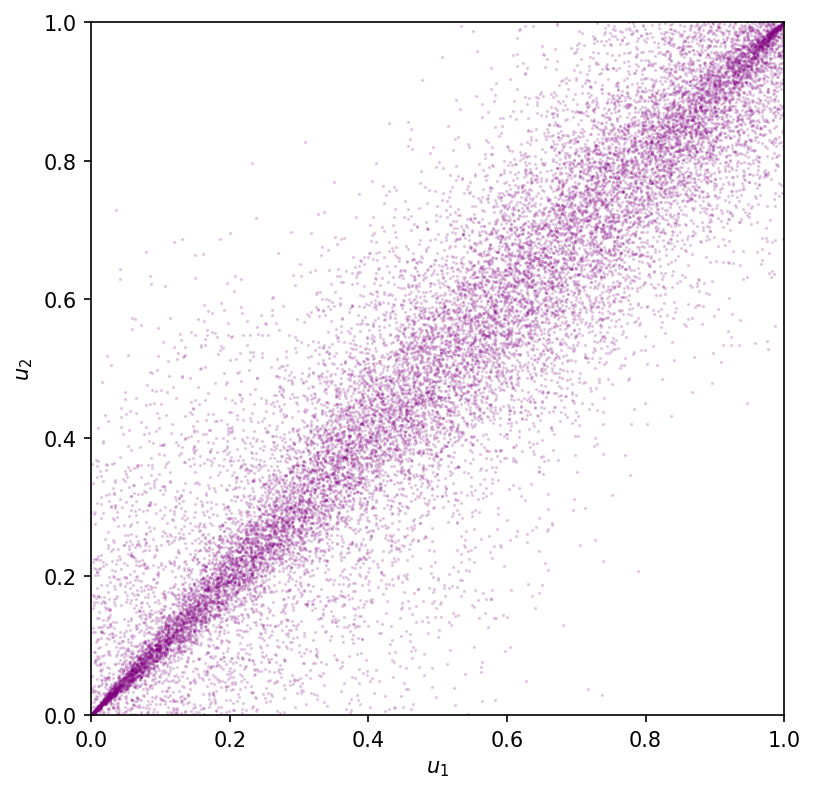
\includegraphics[width=0.65\linewidth]{fig_1d_mixture.png}
\caption{Mixture $0.6\,C^{Cla}_{10}+0.4\,\hat C^{Cla}_{5}$ scatter ($N=10^5$).}
\label{fig:1d}
\end{figure}

\paragraph{Student-$t$ copula log-likelihood (slides eq.\,38).}
Let $y_{it}=t_\nu^{-1}(\hat u_{it})$ and
$Q_t=y_{1t}^2-2\rho y_{1t}y_{2t}+y_{2t}^2$. Then
\begin{align}
\ln c^t(\hat u_{1t},\hat u_{2t};\rho,\nu)
&=\ln\Gamma(\tfrac{\nu+2}{2})+\ln\Gamma(\tfrac{\nu}{2})
   -2\ln\Gamma(\tfrac{\nu+1}{2})-\tfrac12\ln(1-\rho^2)\notag\\
&\quad-\tfrac{\nu+2}{2}\,\ln\!\Bigl(1+\tfrac{Q_t}{\nu(1-\rho^2)}\Bigr)
+\tfrac{\nu+1}{2}\sum_{i=1}^{2}\ln\!\Bigl(1+\tfrac{y_{it}^2}{\nu}\Bigr).
\label{eq:t-cop-ll}
\end{align}
\code{exercise1.estimation.estimate\_t\_copula} maximises this by Nelder--Mead.

\paragraph{Result.} The fitted t-copula returns $\hat\rho=0.929316$, $\hat\nu=2.1698$,
$\ln L=96{,}886.07$. The very small $\hat\nu$ is the t-copula's only way to
mimic the heavy joint tails of the Clayton mixture --- a Gaussian fit on the
same data gives $\hat\rho=0.9057$ and $\ln L=85{,}791$.
This is a textbook example of how IFM correctly
identifies tail dependence by inflating the t-copula degrees of freedom downward.

% =====================================================================
\section{Exercise 2 -- DCC dynamics on cryptocurrency returns}\label{sec:ex2}
% =====================================================================

We work with the daily log-returns of three crypto assets
(BTC, ETH, ADA) loaded from \file{crypto.xlsx}. The sample spans
$T=1827$ trading days from 2 January 2020 to 1 January 2025. The whole pipeline
is in \file{exercise2/} (orchestrated by \file{exercise2/main.py}).

% ---------------------------------------------------------------
\subsection{2.1 -- Univariate descriptives and sample correlations}
% ---------------------------------------------------------------

\begin{table}[H]\centering\small
\caption{Daily log-return descriptives. Skewness uses $b_1$,
kurtosis is the \emph{regular} (non-excess) version.}\label{tab:21-desc}
\begin{tabular}{lrrrr}
\toprule
Asset & Mean & Std & Skew & Kurt\\\midrule
BTC & $0.001404$ & $0.034701$ & $-1.6580$ & $29.3539$\\
ETH & $0.001780$ & $0.044965$ & $-1.3830$ & $23.2127$\\
ADA & $0.001777$ & $0.052556$ & $-0.2361$ & $11.7605$\\
\bottomrule
\end{tabular}
\end{table}

\paragraph{Sample correlation matrix.}
$\rho_{\textsc{btc-eth}}=0.8355$,\quad
$\rho_{\textsc{btc-ada}}=0.6928$,\quad
$\rho_{\textsc{eth-ada}}=0.7353$.

The three series exhibit crypto stylised facts: near-zero mean,
markedly negative skew (especially BTC and ETH), and a pronounced excess
kurtosis (Pearson kurtosis $\gg 3$).

% ---------------------------------------------------------------
\subsection{Theoretical framework: GARCH/GJR + DCC}
% ---------------------------------------------------------------

\paragraph{Marginal volatility -- GARCH(1,1) (slides eq.\,67).}
For a zero-mean return $r_t$,
\begin{equation}\label{eq:garch}
r_t=\sqrt{h_t}\,z_t,\qquad
h_t=\omega+\alpha r_{t-1}^{2}+\beta\,h_{t-1},\qquad z_t\sim\mathcal{N}(0,1)\ \text{i.i.d.}
\end{equation}
Conditions: $\omega>0$, $\alpha,\beta\ge 0$, persistence $\alpha+\beta<1$. The
Gaussian (quasi-) MLE log-likelihood is
\[
\ell(\theta)=-\tfrac12\sum_{t=1}^T\Bigl[\ln(2\pi)+\ln h_t+\frac{r_t^2}{h_t}\Bigr],
\qquad h_1\equiv\widehat{\sigma}_r^{\,2}.
\]
We optimise by L-BFGS-B in \code{exercise2.garch.estimate\_garch}.

\paragraph{Marginal volatility with leverage -- GJR(1,1) (slides eq.\,71).}
\begin{equation}\label{eq:gjr}
h_t=\omega+\bigl(\alpha+\gamma\,\indic\{r_{t-1}<0\}\bigr)r_{t-1}^{2}+\beta\,h_{t-1},
\end{equation}
with persistence $\alpha+\beta+\gamma/2<1$ (because $\Pr(r<0)\approx 1/2$ under
symmetric innovations). $\gamma>0$ captures the leverage effect.

\paragraph{From margins to standardised innovations.}
Let $\hat\eta_{it}$ denote the standardised residual of asset $i$ at time $t$:
\[
\hat\eta_{it}=
\begin{cases}
\Phi^{-1}\!\bigl(\hat F_{i}^{\text{EDF}}(r_{it})\bigr)& \text{(EDF margin, 2.2a)}\\[2pt]
r_{it}/\sqrt{\hat h_{it}}, & \text{(GARCH/GJR margin, 2.2b--c)}.
\end{cases}
\]

\paragraph{DCC dynamics (Engle, 2002 -- slides eqs.\,68--69).}
With $z_t=\hat\eta_t$ (an $n\times 1$ vector of standardised innovations) we
posit
\begin{align}
Q_t &=(1-a-b)\,\hat\Omega+a\,z_{t-1}z_{t-1}^\top+b\,Q_{t-1},\quad Q_1=\hat\Omega,\label{eq:dcc-Q}\\
\Psi_t &=\Lambda_t^{-1/2}\,Q_t\,\Lambda_t^{-1/2},\qquad \Lambda_t=\diag(Q_t),\label{eq:dcc-psi}
\end{align}
where $\hat\Omega=\frac{1}{T}\sum_t z_tz_t^\top$ and $a,b>0$, $a+b<1$. The
normalisation in \eqref{eq:dcc-psi} ensures $\Psi_t$ is a correlation matrix.

\paragraph{Gaussian DCC log-likelihood (slides eq.\,72).}
The copula likelihood (margins concentrated out) is
\begin{equation}\label{eq:dcc-LL-G}
\ell^G(a,b)=-\tfrac12\sum_{t=1}^{T}\Bigl[\ln|\Psi_t|+\eta_t^\top(\Psi_t^{-1}-I_n)\eta_t\Bigr].
\end{equation}

\paragraph{Student-$t$ DCC log-likelihood (slides eq.\,76).}
With $A(\nu)=\dfrac{\Gamma\!\bigl(\tfrac{\nu+n}{2}\bigr)\,\Gamma\!\bigl(\tfrac{\nu}{2}\bigr)^{n-1}}
{\Gamma\!\bigl(\tfrac{\nu+1}{2}\bigr)^{n}}$,
\begin{align}
\ell^t(a,b,\nu)
&=T\ln A(\nu)-\tfrac12\sum_{t}\ln|\Psi_t|
   -\tfrac{\nu+n}{2}\sum_t\ln\!\Bigl(1+\tfrac{1}{\nu}\eta_t^\top\Psi_t^{-1}\eta_t\Bigr)\notag\\
&\quad+\tfrac{\nu+1}{2}\sum_t\sum_{i=1}^n\ln\!\Bigl(1+\tfrac{\eta_{it}^2}{\nu}\Bigr),
\label{eq:dcc-LL-t}
\end{align}
with $\eta_{it}=t_\nu^{-1}(\hat u_{it})$ obtained from the EDF margins. Both
likelihoods are maximised by Nelder--Mead in \code{exercise2.dcc}.

% ---------------------------------------------------------------
\subsection{2.2 -- DCC under three marginal specifications}
% ---------------------------------------------------------------

\paragraph{(a) EDF margins.} $\hat a=0.012308$, $\hat b=0.987592$, $\hat a+\hat
b=0.999900$, $\ln L=1954.19$, with unconditional correlations
$\hat\Omega_{\textsc{btc-eth}}=0.8248$, $\hat\Omega_{\textsc{btc-ada}}=0.7039$,
$\hat\Omega_{\textsc{eth-ada}}=0.7418$. The persistence is essentially 1.
See Figure~\ref{fig:22a}.

\begin{figure}[H]\centering
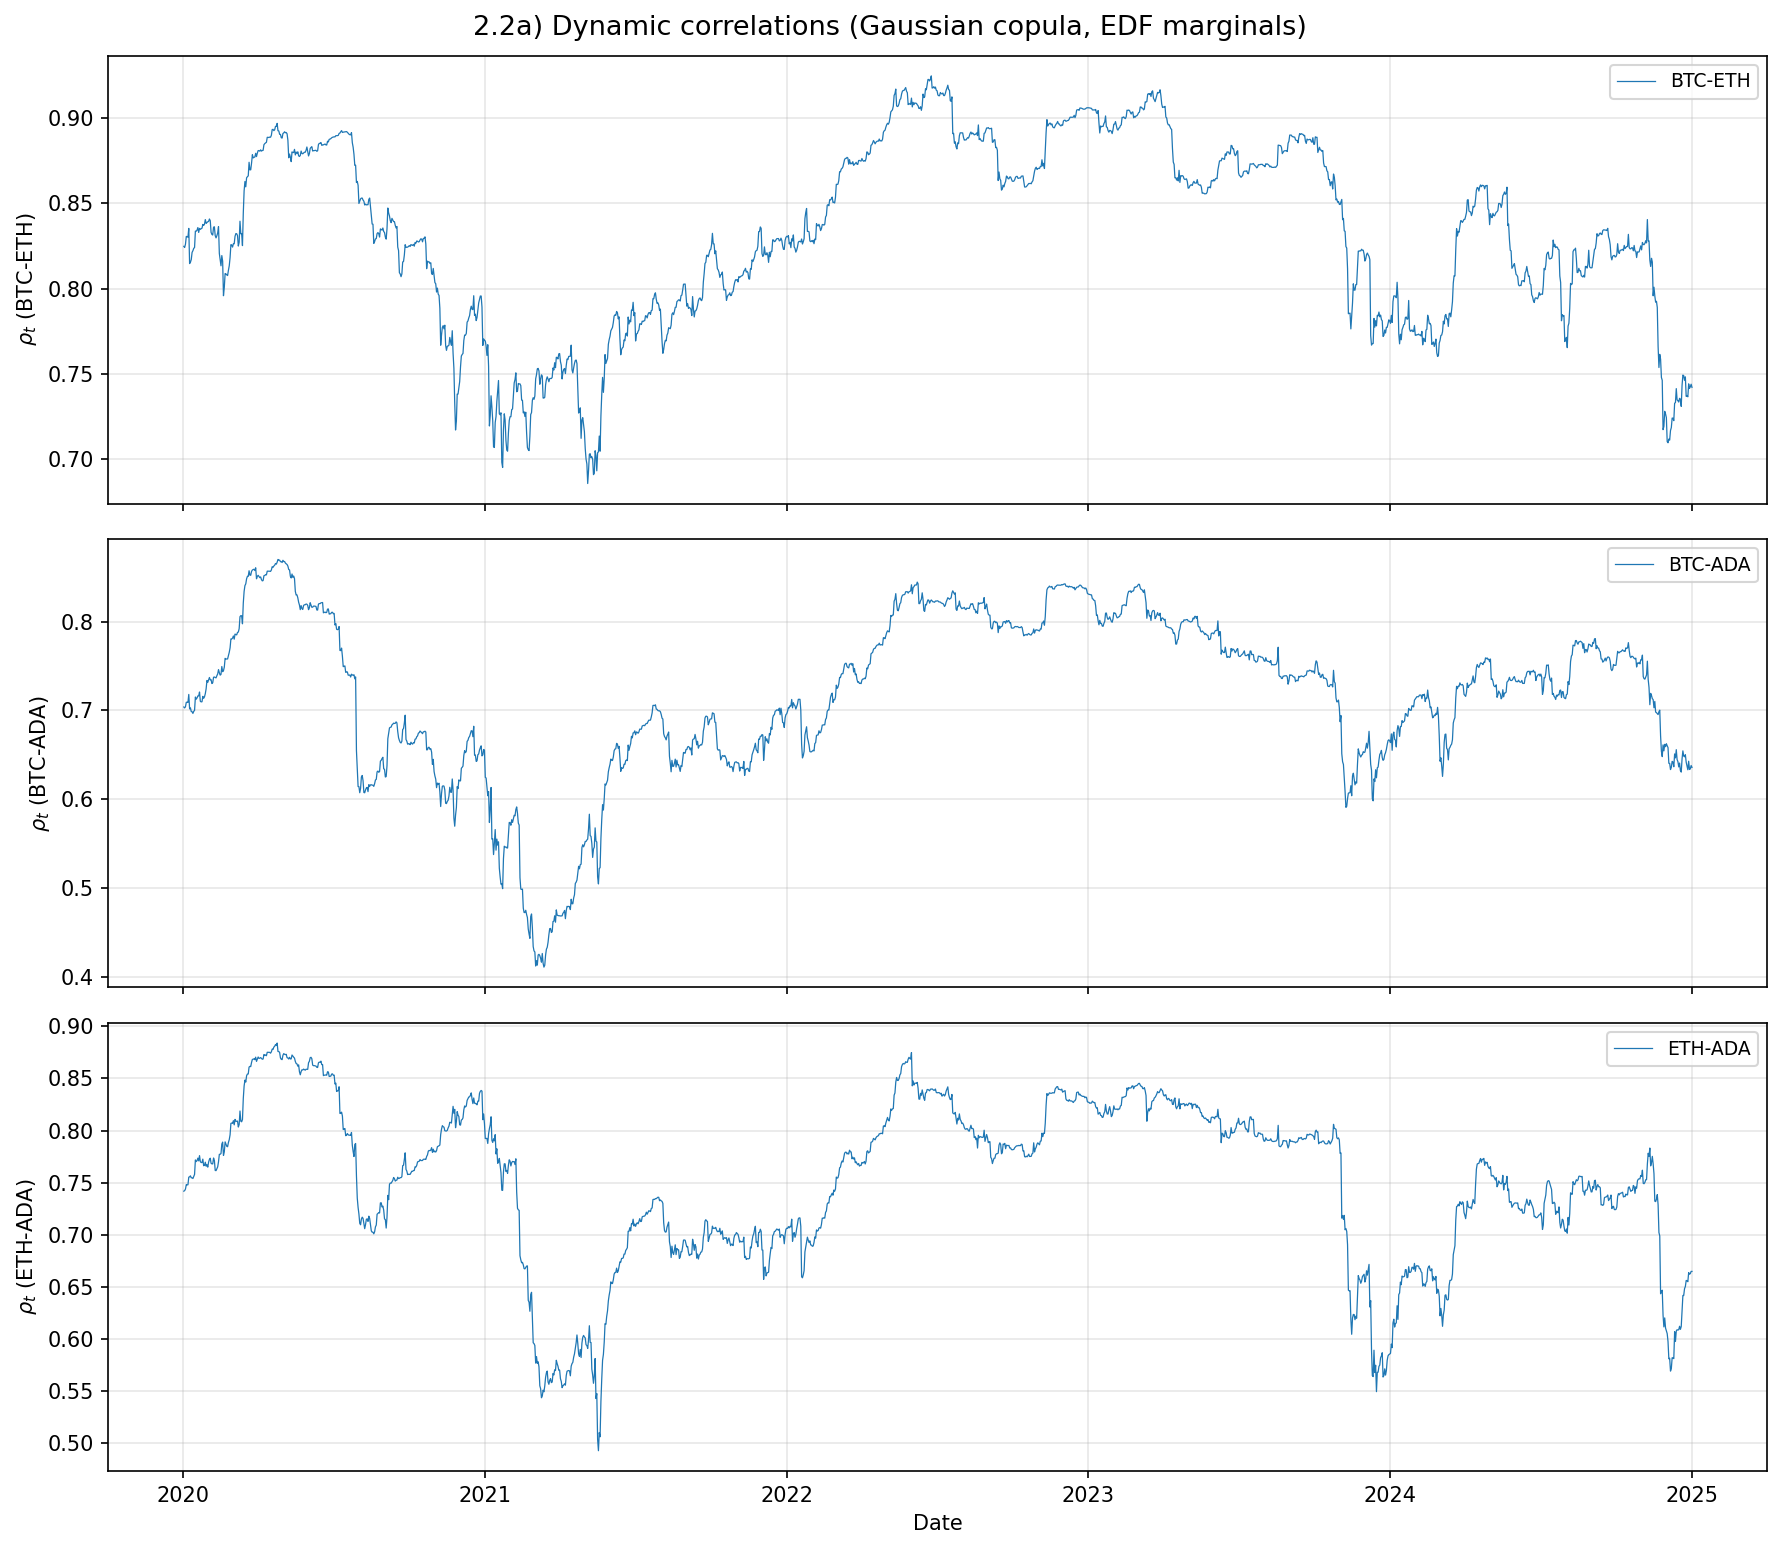
\includegraphics[width=0.85\linewidth]{fig_2_2a_dcc_edf.png}
\caption{Dynamic correlations under DCC-Gaussian with EDF margins.}\label{fig:22a}
\end{figure}

\newpage
\paragraph{(b) GARCH(1,1)-N margins.} The marginal estimates are reported in
Table~\ref{tab:22b-margins}. The DCC stage gives $\hat a=0.060304$,
$\hat b=0.900190$, $\hat a+\hat b=0.960494$, $\ln L=1964.18$.

\begin{table}[H]\centering\small
\caption{GARCH(1,1)-N marginal estimates.}\label{tab:22b-margins}
\begin{tabular}{lrrrrr}
\toprule
Asset & $\omega$ & $\alpha$ & $\beta$ & $\alpha+\beta$ & $\ln L$\\\midrule
BTC & $4.88\times 10^{-5}$ & $0.1146$ & $0.8595$ & $0.9741$ & $5324.93$\\
ETH & $3.95\times 10^{-5}$ & $0.1030$ & $0.8850$ & $0.9880$ & $4943.94$\\
ADA & $1.11\times 10^{-4}$ & $0.1365$ & $0.8336$ & $0.9701$ & $4633.55$\\
\bottomrule
\end{tabular}
\end{table}

\begin{figure}[H]\centering
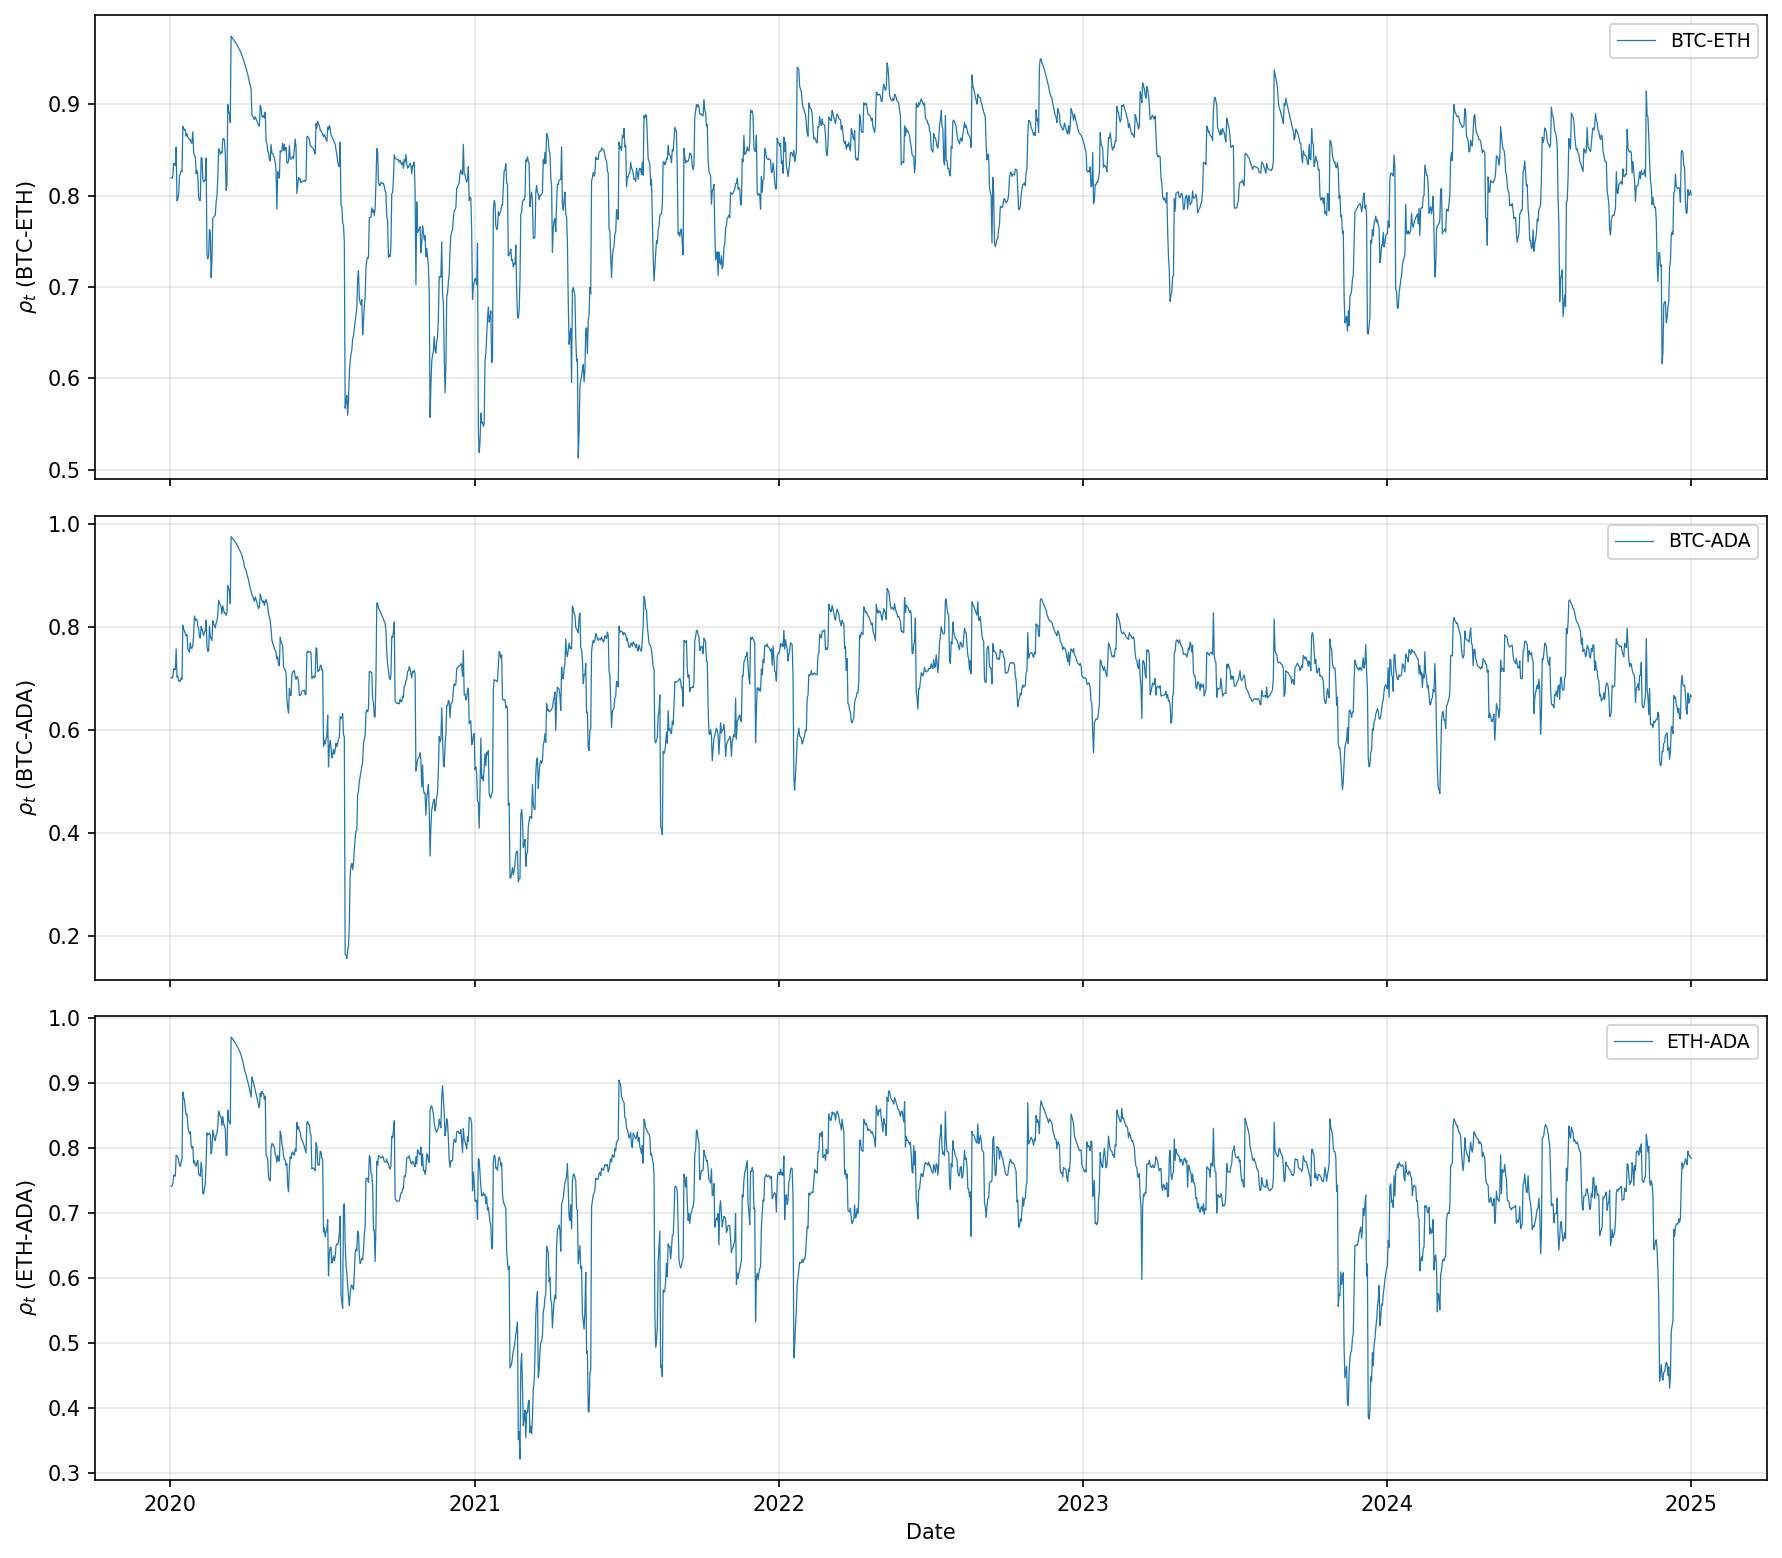
\includegraphics[width=0.85\linewidth]{fig_2_2b_dcc_garch.png}
\caption{DCC dynamic correlations with GARCH(1,1)-N margins.}\label{fig:22b}
\end{figure}

\paragraph{(c) GJR(1,1)-N margins.}
Table~\ref{tab:22c-margins}. DCC parameters: $\hat a=0.062861$, $\hat b=0.902904$,
$\hat a+\hat b=0.965765$, $\ln L=1934.41$.

\begin{table}[H]\centering\small
\caption{GJR(1,1)-N marginal estimates. $\gamma$ is the leverage coefficient.}
\label{tab:22c-margins}
\begin{tabular}{lrrrrr}
\toprule
Asset & $\alpha$ & $\beta$ & $\gamma$ & Persistence & $\ln L$\\\midrule
BTC & $0.0713$ & $0.8426$ & $0.0996$ & $0.9637$ & $5340.71$\\
ETH & $0.0852$ & $0.8776$ & $0.0457$ & $0.9857$ & $4946.55$\\
ADA & $0.1288$ & $0.8280$ & $0.0265$ & $0.9701$ & $4634.15$\\
\bottomrule
\end{tabular}
\end{table}

\begin{figure}[H]\centering
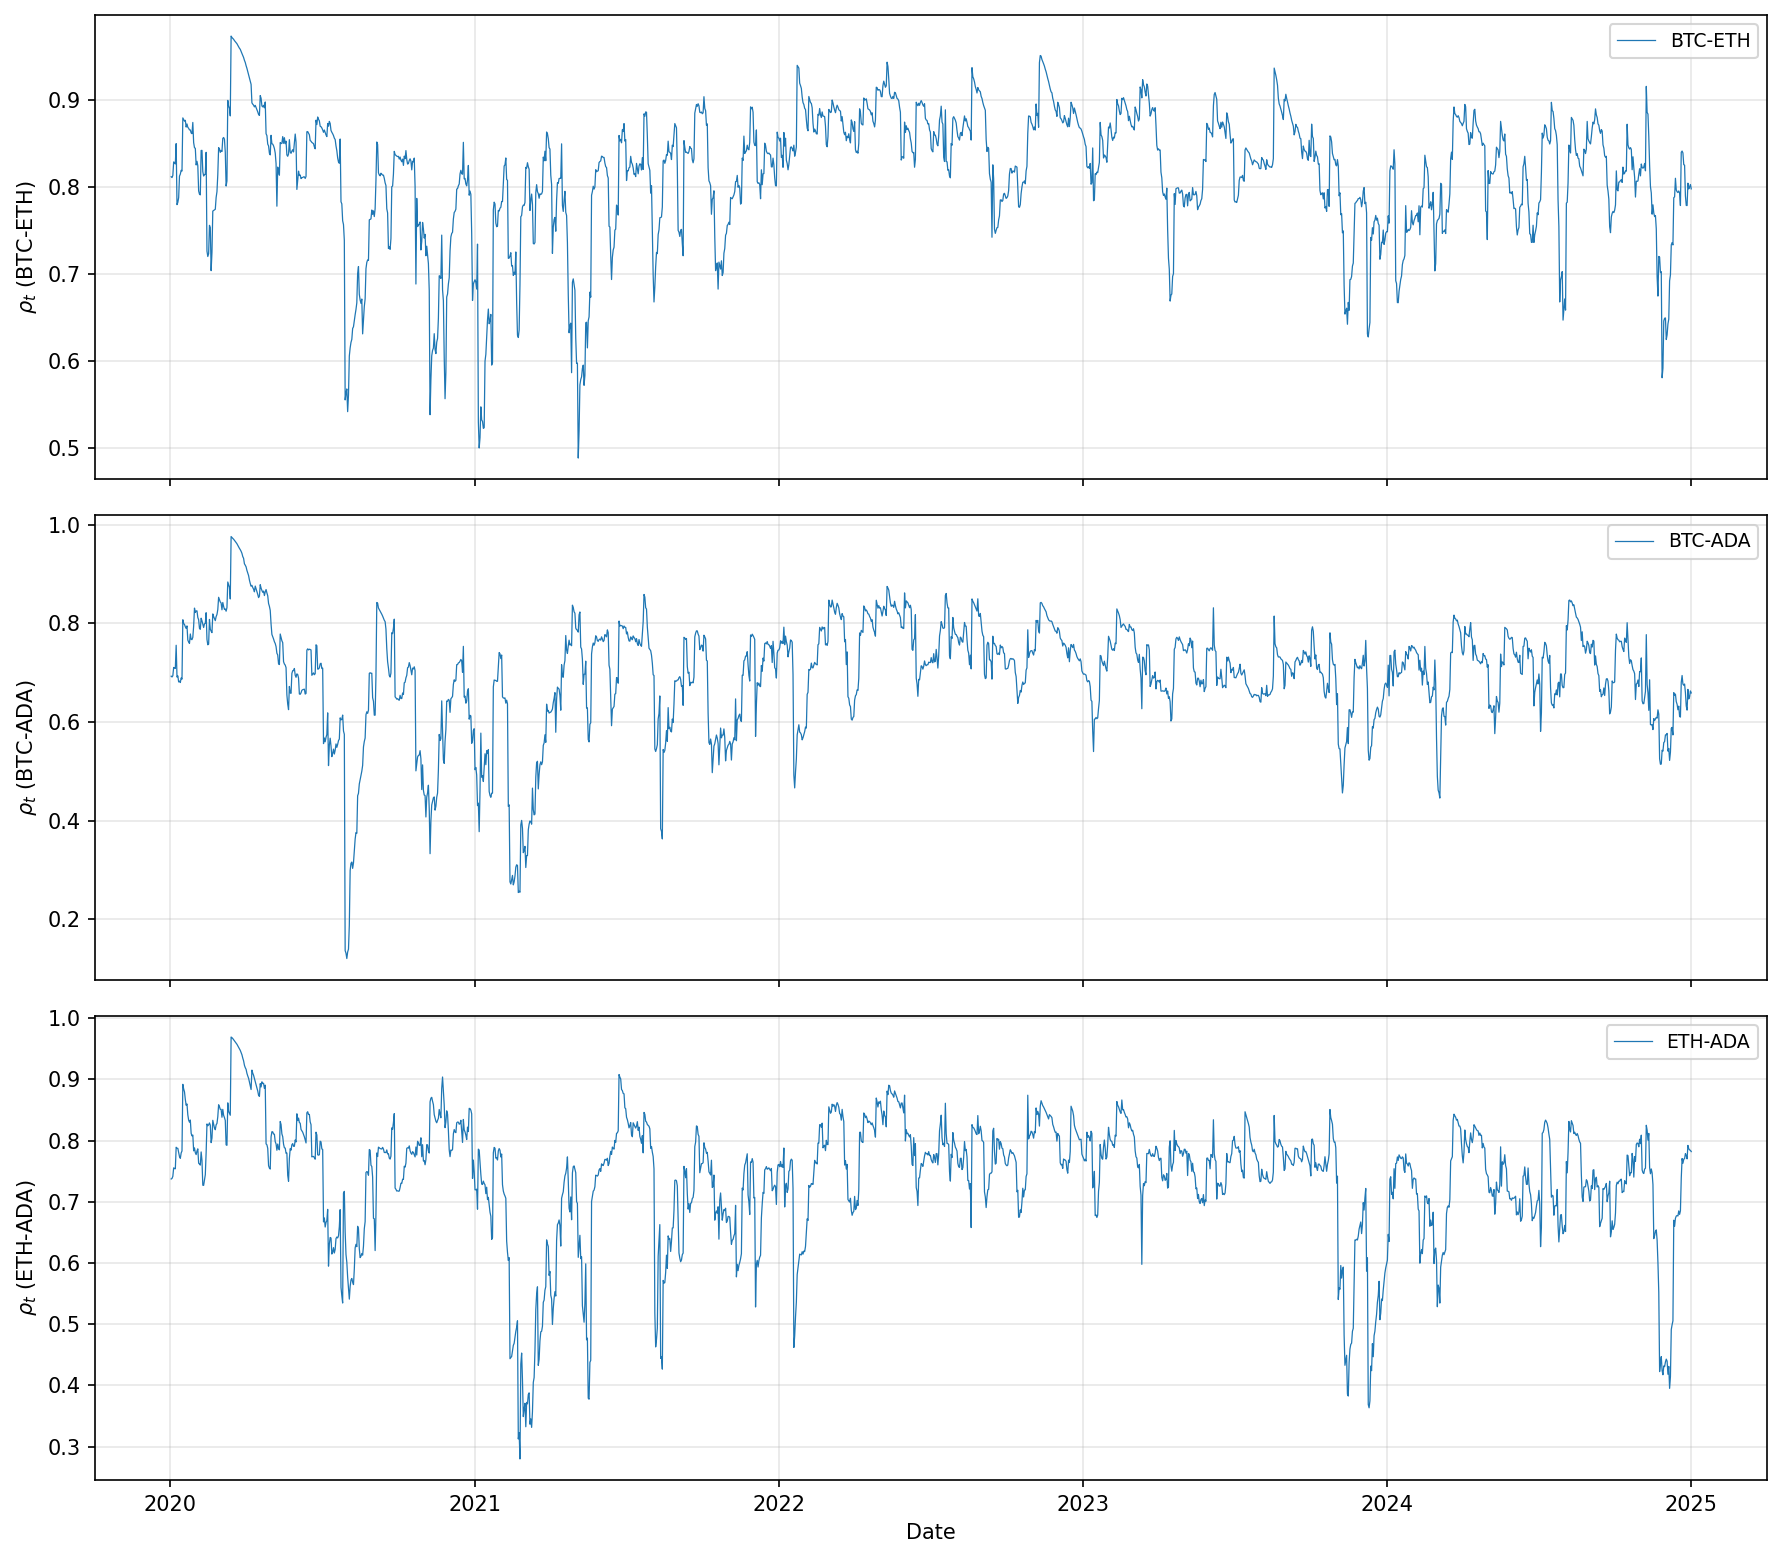
\includegraphics[width=0.85\linewidth]{fig_2_2c_dcc_gjr.png}
\caption{DCC dynamic correlations with GJR(1,1)-N margins.}\label{fig:22c}
\end{figure}

% ---------------------------------------------------------------
\subsection{2.3 -- Comparison of dynamic correlation paths}
% ---------------------------------------------------------------

Figure~\ref{fig:23} overlays the three correlation paths for the
three marginal specifications. Table~\ref{tab:23-summary} summarises the
sample distribution of each path.

\begin{table}[H]\centering\small
\caption{Distribution of estimated dynamic correlations across $T=1827$ days.}
\label{tab:23-summary}
\begin{tabular}{llrrrr}
\toprule
Pair & Margin & Mean & Std & Min & Max\\\midrule
\multirow{3}{*}{BTC--ETH}
 & EDF      & $0.8333$ & $0.0538$ & $0.6857$ & $0.9248$\\
 & GARCH-N  & $0.8200$ & $0.0700$ & $0.5129$ & $0.9746$\\
 & GJR-N    & $0.8148$ & $0.0751$ & $0.4887$ & $0.9731$\\\midrule
\multirow{3}{*}{BTC--ADA}
 & EDF      & $0.7187$ & $0.0917$ & $0.4114$ & $0.8697$\\
 & GARCH-N  & $0.7012$ & $0.1051$ & $0.1564$ & $0.9751$\\
 & GJR-N    & $0.6962$ & $0.1132$ & $0.1207$ & $0.9761$\\\midrule
\multirow{3}{*}{ETH--ADA}
 & EDF      & $0.7511$ & $0.0779$ & $0.4928$ & $0.8839$\\
 & GARCH-N  & $0.7410$ & $0.0977$ & $0.3218$ & $0.9706$\\
 & GJR-N    & $0.7388$ & $0.1042$ & $0.2796$ & $0.9692$\\
\bottomrule
\end{tabular}
\end{table}

\begin{figure}[H]\centering
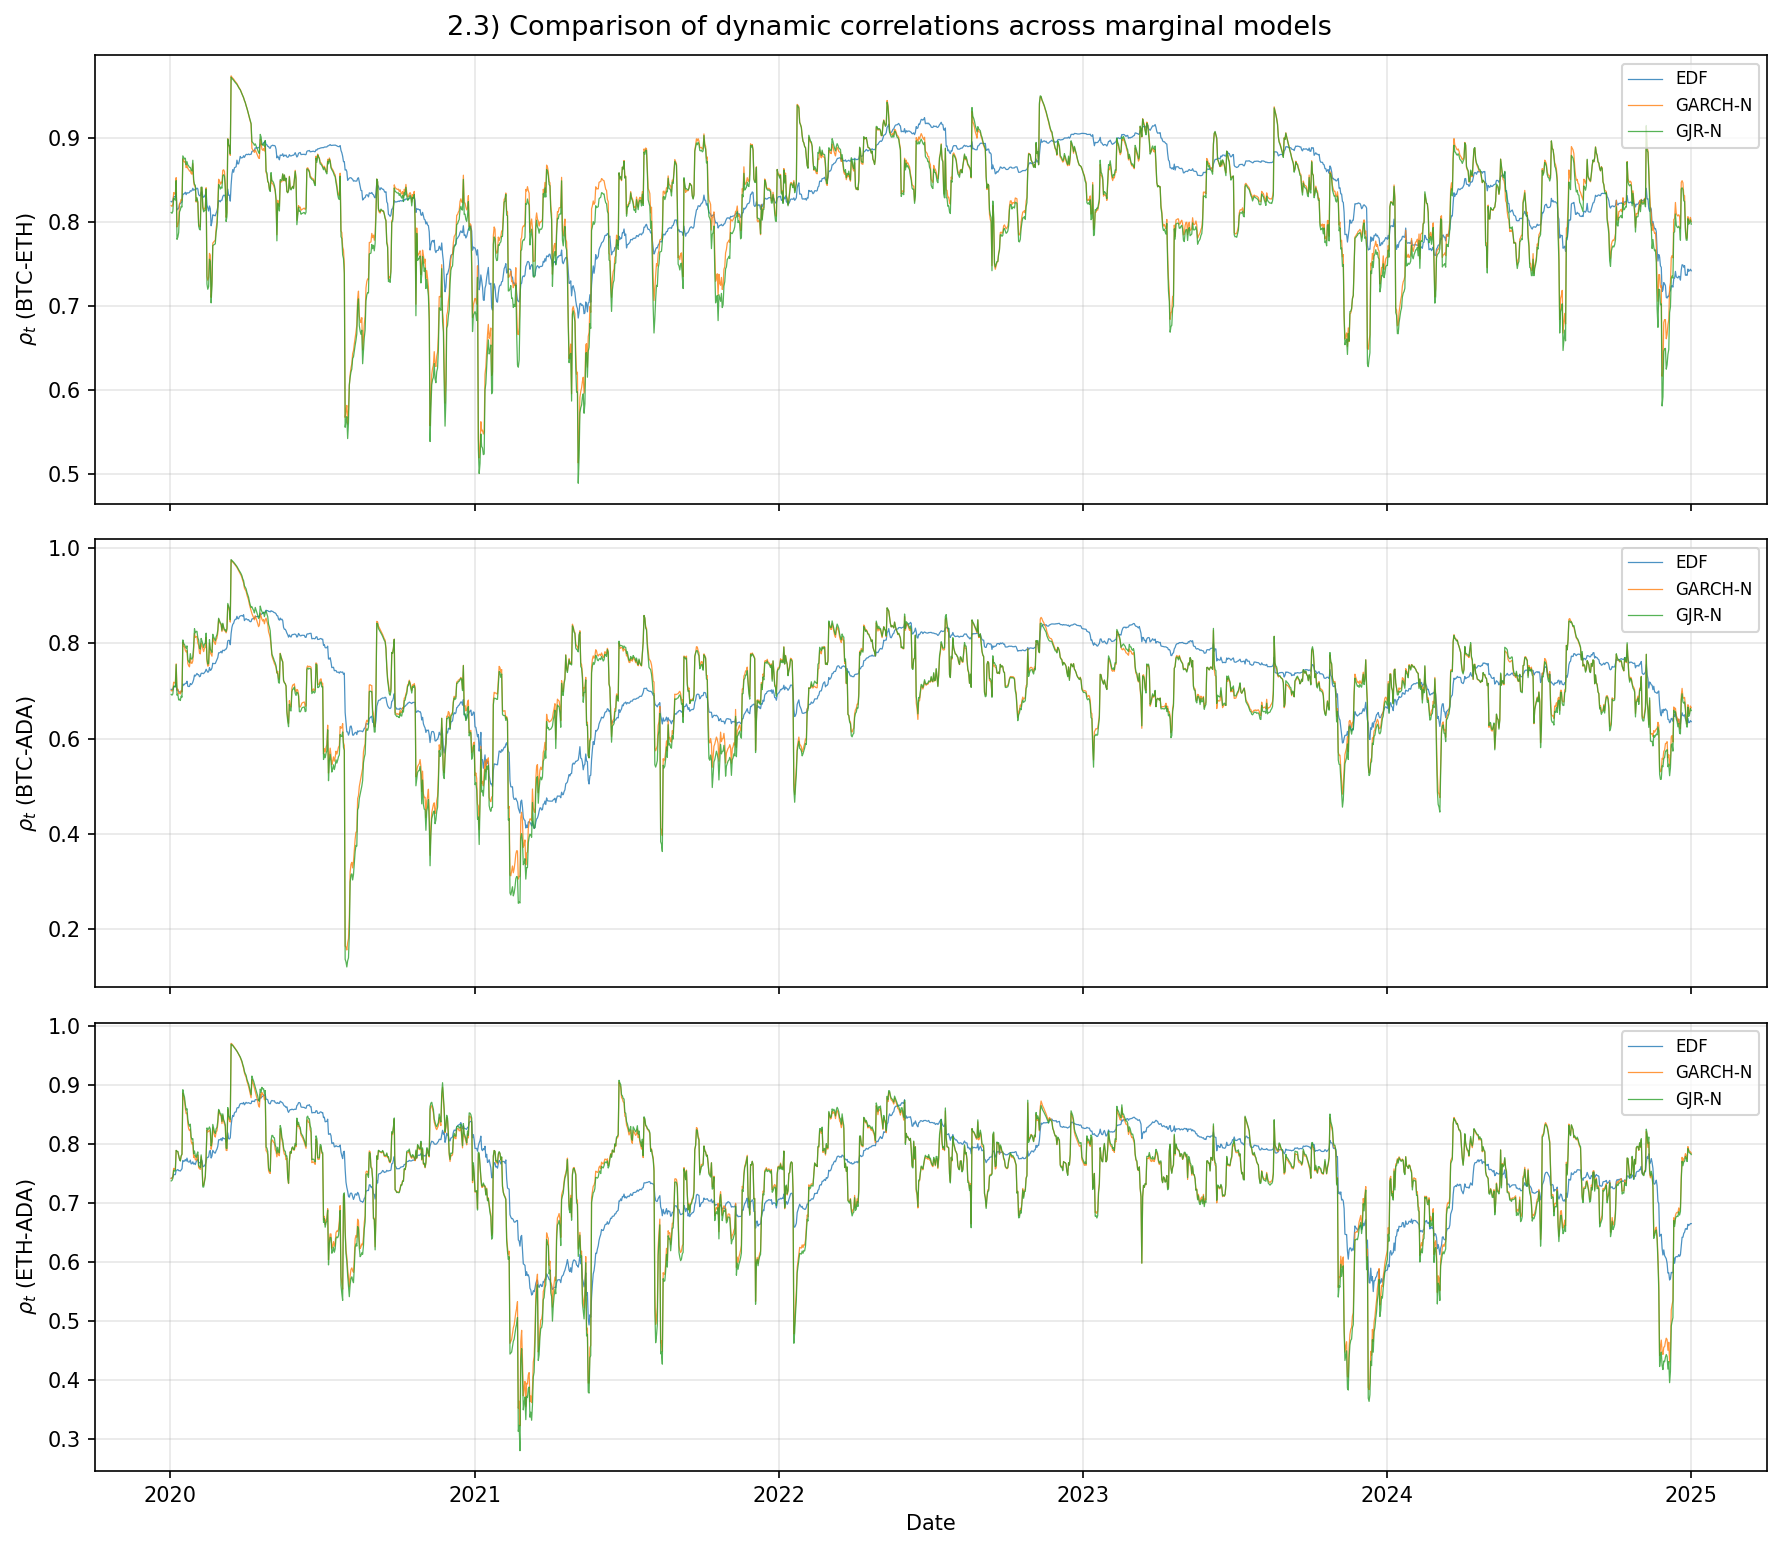
\includegraphics[width=0.95\linewidth]{fig_2_3_comparison.png}
\caption{Pair-wise dynamic correlations under EDF, GARCH-N, and GJR-N margins.}
\label{fig:23}
\end{figure}

\paragraph{Reading the comparison.}
The three series share the same pattern, correlations rise
during shocks as the COVID-19 shock (March 2020). Quantitatively, EDF
produces the smoothest path, while GARCH/GJR capture sharper short-run drops in
dependence. The $\hat a+\hat b$ estimate falls from $0.9999$ (EDF) to $\approx
0.96$ once the marginal variance is filtered.

% ---------------------------------------------------------------
\subsection{2.4 -- DCC under a Student-$t$ copula (EDF margins)}
% ---------------------------------------------------------------

We now jointly estimate $(a,b,\nu)$ in \eqref{eq:dcc-LL-t}. The estimates are
$\hat a=0.039216$, $\hat b=0.937845$, $\hat\nu=4.3936$, $\ln L=2093.03$. The
LL gain over the Gaussian-EDF specification is $2093.03-1954.19=138.84$,
overwhelming evidence that the joint tail of the three crypto returns is
heavier than Gaussian and well captured by a $t$-copula with around four
degrees of freedom. Figure~\ref{fig:24} reports the dynamic correlations.

\begin{figure}[H]\centering
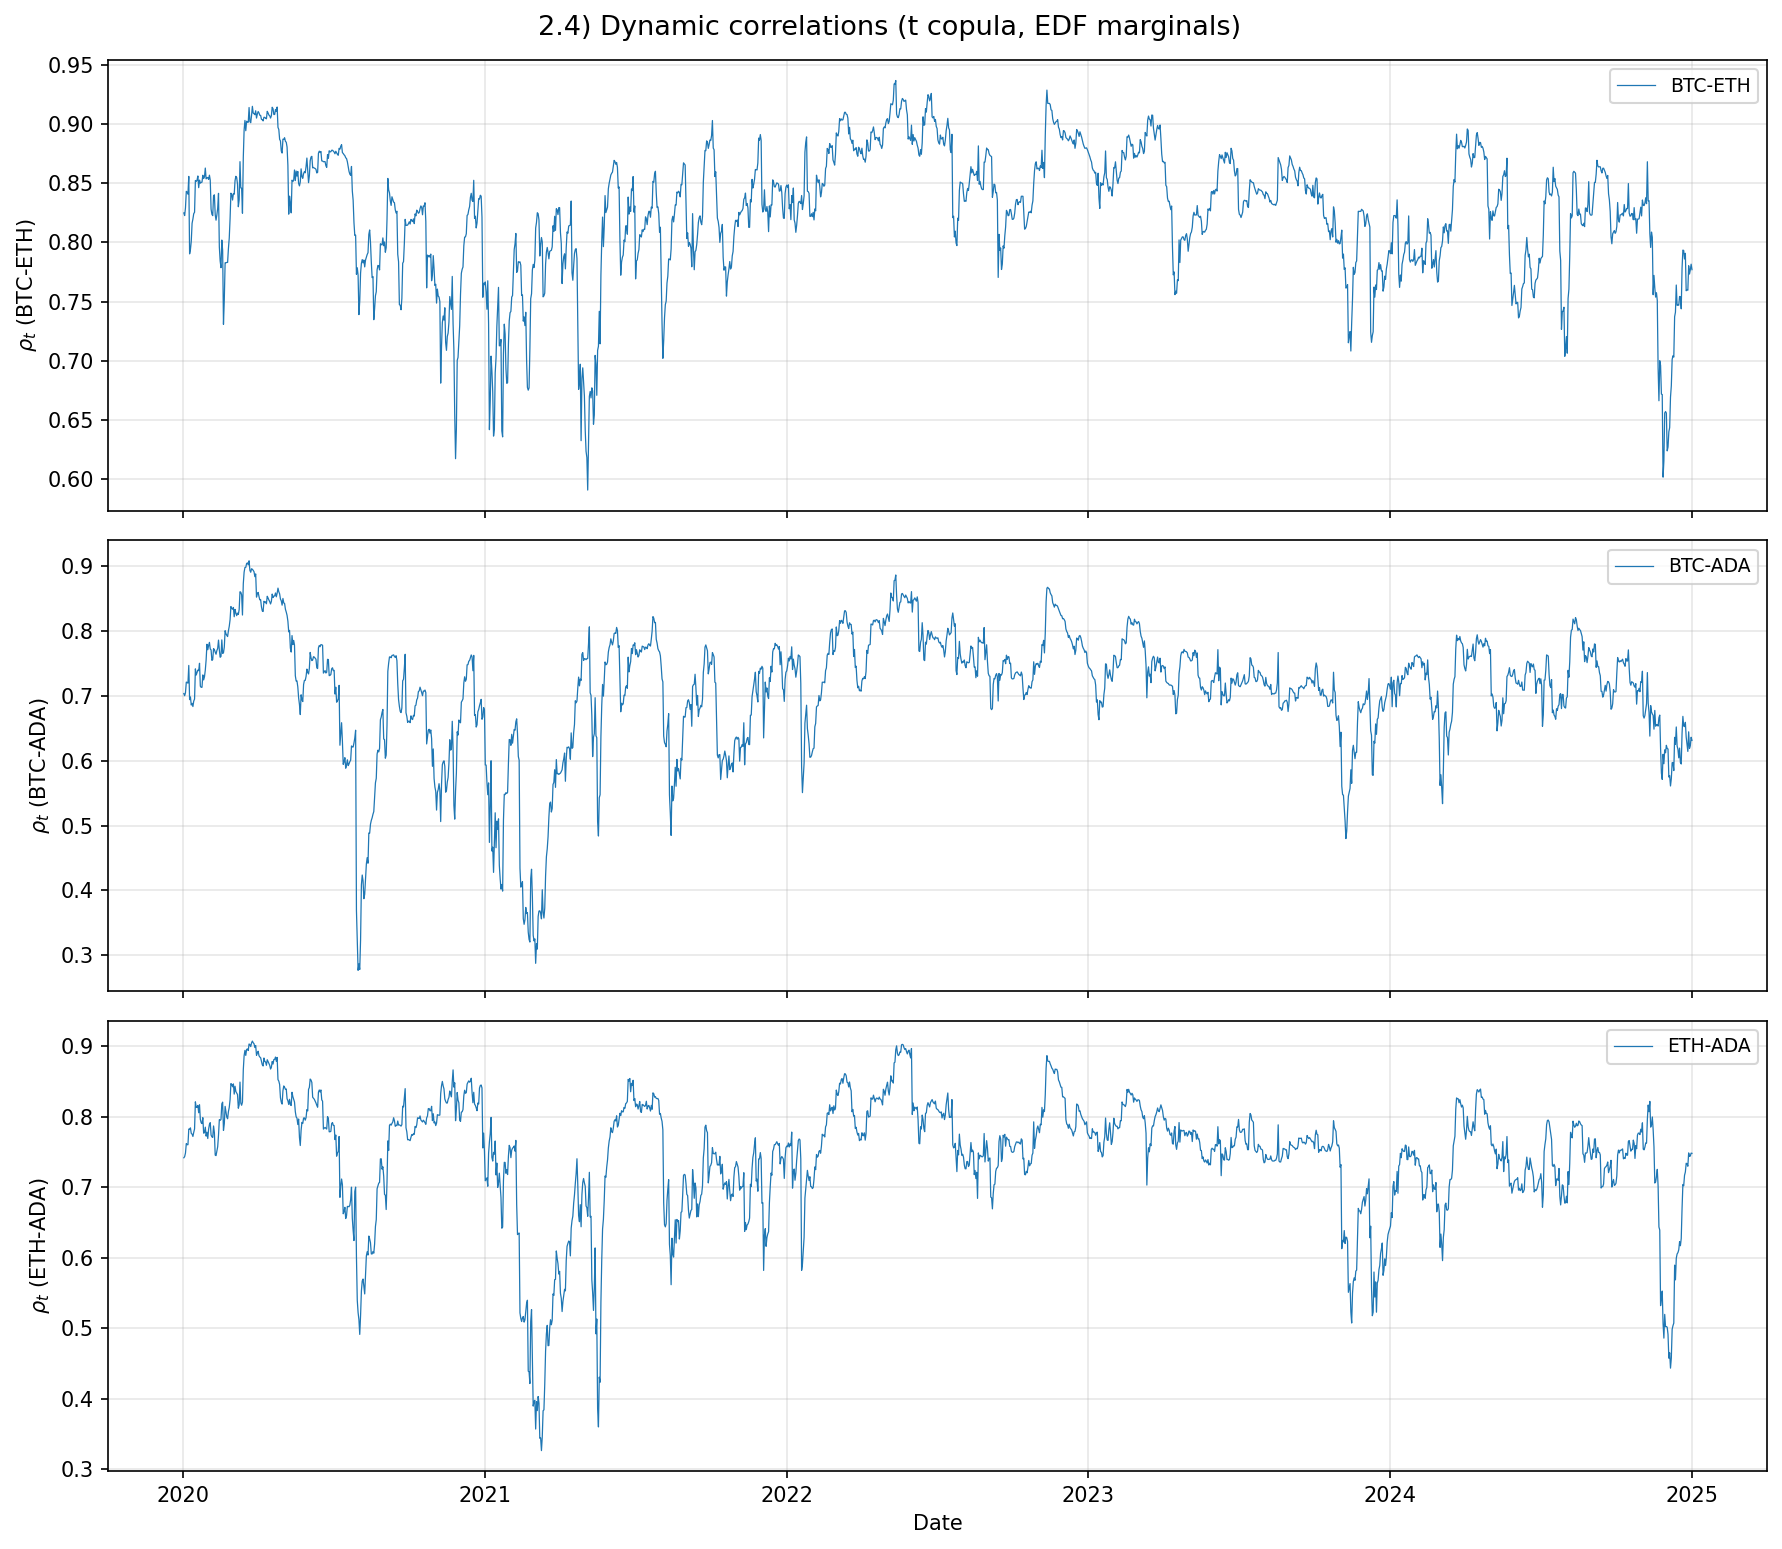
\includegraphics[width=0.85\linewidth]{fig_2_4_dcc_t.png}
\caption{Dynamic correlations under DCC-$t$ copula with EDF margins
($\hat\nu=4.39$).}\label{fig:24}
\end{figure}

\paragraph{Intuition for $\hat\nu\approx 4.4$.}
A finite $\nu$ is the device by which the Student-$t$ copula introduces
\emph{tail dependence} (absent in the Gaussian copula). With three crypto
assets sharing common shocks during stress periods, $\hat\nu$ is pushed
toward small values; values in the 4--6 range are typical of equity
indices, and the crypto evidence here lies just at the lower end of that range.

% =====================================================================
\section{Exercise 3 -- Conditional quantile curves of the NM copula}\label{sec:ex3}
% =====================================================================

% ---------------------------------------------------------------
\subsection{Specification}
% ---------------------------------------------------------------

The Normal-Mixture (NM) copula is the convex combination of two Gaussian
copulas with different correlations:
\[
C^{NM}(u_1,u_2)=\pi\,C^G_{\rho_1}(u_1,u_2)+(1-\pi)\,C^G_{\rho_2}(u_1,u_2),
\quad 0<\pi<1.
\]
Since the conditional CDF is linear in the components, the conditional NM CDF
inherits the same structure:
\begin{equation}\label{eq:nm-cond}
C^{NM}(u_1\given u_2)
=\pi\,\Phi\!\Bigl(\tfrac{\Phi^{-1}(u_1)-\rho_1\Phi^{-1}(u_2)}{\sqrt{1-\rho_1^2}}\Bigr)
+(1-\pi)\,\Phi\!\Bigl(\tfrac{\Phi^{-1}(u_1)-\rho_2\Phi^{-1}(u_2)}{\sqrt{1-\rho_2^2}}\Bigr).
\end{equation}
Parameters used: $\pi=\ExThreePi,\;\rho_1=\ExThreeRhoA,\;\rho_2=\ExThreeRhoB$.

% ---------------------------------------------------------------
\subsection{Definition of $q$-quantile curves}
% ---------------------------------------------------------------

For each conditioning value $u_2\in(0,1)$ and each level $q\in(0,1)$ the
$q$-quantile curve is the locus
\[
\bigl\{(u_2,u_1)\in(0,1)^2 : C^{NM}(u_1\given u_2)=q\bigr\}.
\]
Because $u_1\mapsto C^{NM}(u_1\given u_2)$ is a CDF on $(0,1)$ (hence
\emph{strictly increasing} from 0 to 1), the equation has a unique root for
every $q\in(0,1)$. We solve it by Brent's method on $[\varepsilon,1-\varepsilon]$
with $\varepsilon=10^{-4}$ in
\code{exercise3.nm\_copula.nm\_quantile\_u1}.

\begin{remark}[Why we invert in $u_1$ and not in $u_2$]
The reading of the problem statement asks to obtain $u_2$
given $u_1$. However, with $\pi=\ExThreePi$, $\rho_1=\ExThreeRhoA$, $\rho_2=\ExThreeRhoB$ the map
$u_2\mapsto C^{NM}(u_1\given u_2)$ has range bounded inside $(0.3,0.7)$ for a
fixed $u_1$ in the interior, so no $u_2$-solution exists for $q\in\{0.05,0.95\}$.
Consistently with the slides we invert in $u_1$, which has range $(0,1)$ and a unique
solution for every $q$.
\end{remark}

% ---------------------------------------------------------------
\subsection{Numerical results}
% ---------------------------------------------------------------

Table~\ref{tab:3-u1} reports $\hat u_1(u_2;q)$ on a representative grid;
all roots verify $|C^{NM}(\hat u_1\given u_2)-q|<10^{-10}$.
Figure~\ref{fig:3} shows the curves on the $(u_2,u_1)$ unit square (left)
and on the $\mathcal{N}(0,1)$ return scale $(r_2,r_1)=(\Phi^{-1}u_2,\Phi^{-1}u_1)$
(right).

\begin{table}[H]\centering\small
\caption{$\hat u_1$ such that $C^{NM}(\hat u_1\given u_2)=q$.}\label{tab:3-u1}
\begin{tabular}{cccccc}
\toprule
\ExThreeQuantileHeader
\midrule
\ExThreeQuantileBody
\bottomrule
\end{tabular}
\end{table}

\begin{figure}[H]\centering
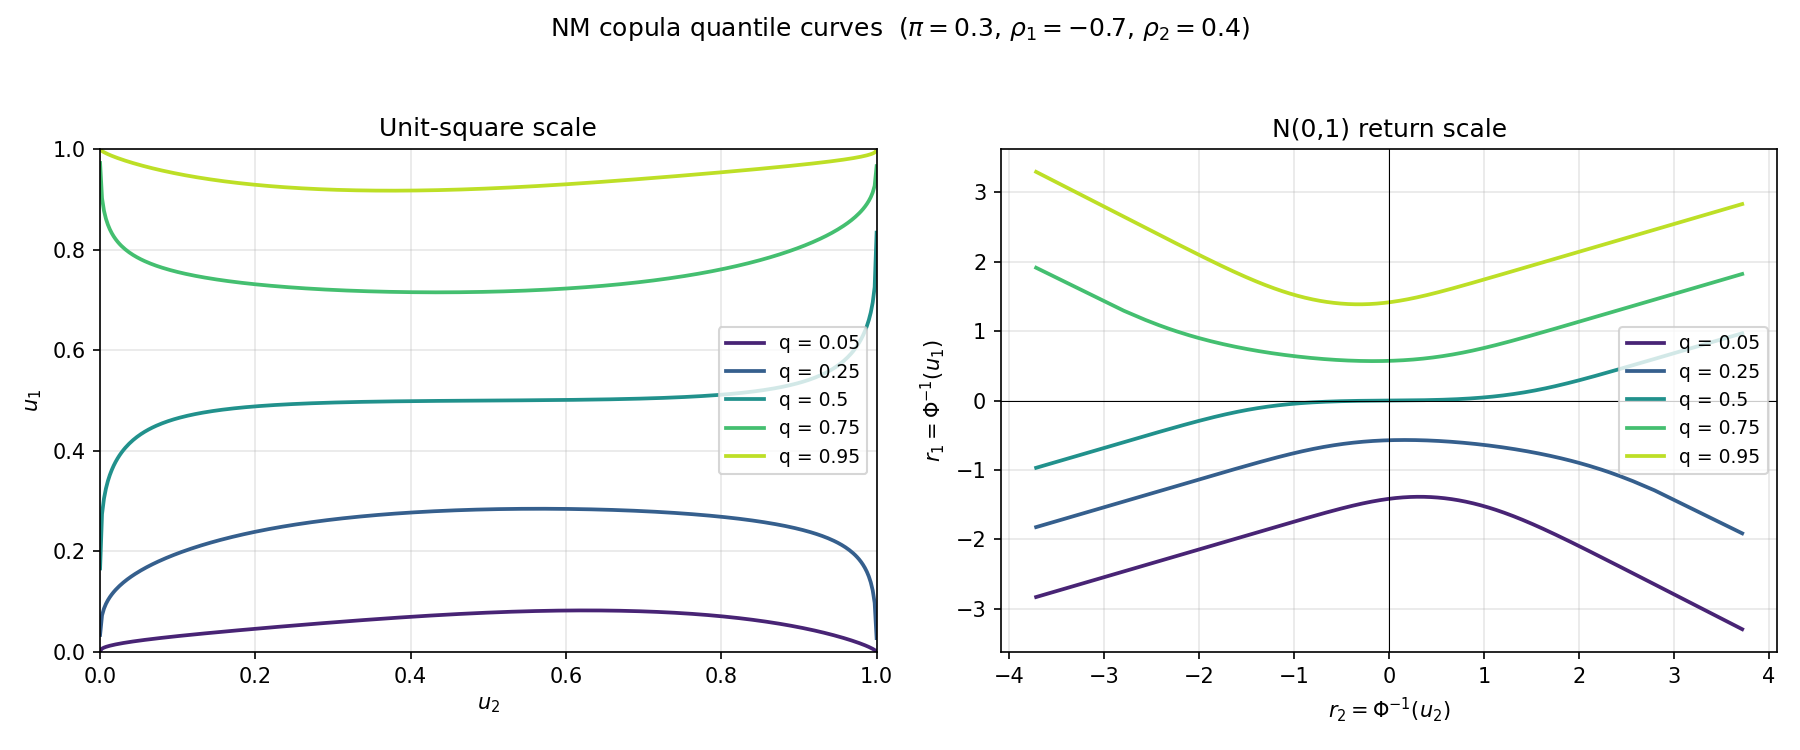
\includegraphics[width=\linewidth]{fig_3_nm_quantile_curves.png}
\caption{NM-copula $q$-quantile curves on the $(u_2,u_1)$ unit square (left)
and on the $\mathcal{N}(0,1)$ return scale (right). Parameters
$\pi=\ExThreePi$, $\rho_1=\ExThreeRhoA$, $\rho_2=\ExThreeRhoB$.}
\label{fig:3}
\end{figure}

\paragraph{Intuition.}
The median curve ($q=0.5$) is symmetric about $u_2=0.5$ because, by
construction, the conditional median of a continuous copula passes through
$(0.5,0.5)$. The outer quantiles are visibly asymmetric: in the lower region ($u_2$ small) the
$q=0.05$ branch is close to zero by the negative-correlation ($\rho_1=\ExThreeRhoA$, weight $\ExThreePi$);
in the positive region ($u_2$ large) the $q=0.05$ quantile is lifted because the positive-correlation
($\rho_2=\ExThreeRhoB$) component dominates. The mixture therefore generates a non-monotone,
``bow-shaped'' tail behaviour.

% =====================================================================
\section{Exercise 4 -- Option-based portfolios under alternative copulas}
\label{sec:ex4}
% =====================================================================

This exercise reproduces the Monte-Carlo experiment of the
\emph{Option-based portfolios} slides (pages 16--19) using a Python port of
\file{ccK\_simuRet2.m}. The full implementation is in \file{exercise4/}.

% ---------------------------------------------------------------
\subsection{Setup}
% ---------------------------------------------------------------

Two assets with log-normal terminal prices
\[
S_{iT}=S_{i0}\exp\!\Bigl(\bigl(\mu-\tfrac12\sigma^2\bigr)T+\sigma\sqrt{T}\,Z_i\Bigr),
\qquad i=1,2,
\]
where $S_{10}=S_{20}=100$, $r=0.03$, $\mu=0.08$, $\sigma=0.2$, $T=1$, and
$(Z_1,Z_2)$ has $\mathcal{N}(0,1)$ marginals coupled by one of four copulas
(scenarios 4.1--4.4 below). $N=10^5$ paths and a strike grid
$K\in\{85,86,\ldots,115\}$.

\paragraph{Black--Scholes prices (port of \file{BS.m}).}
\[
d_1=\frac{\ln(S_0/K)+\bigl(r+\tfrac12\sigma^2\bigr)T}{\sigma\sqrt T},\quad
d_2=d_1-\sigma\sqrt T,
\]
\[
C_0(K,T)=S_0\Phi(d_1)-Ke^{-rT}\Phi(d_2),\qquad
P_0(K,T)=Ke^{-rT}\Phi(-d_2)-S_0\Phi(-d_1).
\]

\paragraph{Portfolio returns.}
We consider four standard strategies (slides eqs.~4--5):
\begin{align}
R_{\text{cc}}(K,T) &=\frac{S_{1T}-\max(S_{1T}-K,0)}{S_{10}-C_0(K,T)}-1
&&\text{(covered call, single asset)}\\
R_{\text{cc2}}(K,T)&=\frac{S_{2T}-\max(S_{1T}-K,0)}{S_{20}-C_0(K,T)}-1
&&\text{(covered call, hedged with asset 1)}\\
R_{\text{pp}}(K,T) &=\frac{S_{1T}+\max(K-S_{1T},0)}{S_{10}+P_0(K,T)}-1
&&\text{(protective put, single asset)}\\
R_{\text{pp2}}(K,T)&=\frac{S_{2T}+\max(K-S_{1T},0)}{S_{20}+P_0(K,T)}-1
&&\text{(protective put, hedged with asset 1)}
\end{align}
\code{cc} and \code{pp} use only $S_{1T}$ and are therefore
\emph{copula-independent}; \code{cc2} and \code{pp2} mix $S_{1T}$ and $S_{2T}$
and so depend on the joint distribution. This is the central distinction the
slides emphasise.

\paragraph{Generation of $(Z_1,Z_2)$.}
\begin{itemize}\setlength\itemsep{0pt}
\item Gaussian copula: direct Cholesky $Z_1=\varepsilon_1$, $Z_2=\rho\varepsilon_1+\sqrt{1-\rho^2}\,\varepsilon_2$.
\item Student-$t$ copula: simulate $(U_1,U_2)\sim C^t_{\rho,\nu}$ via \eqref{eq:t-sim}
      then $Z_i=\Phi^{-1}(U_i)$.
\item Clayton copula: simulate $(U_1,U_2)\sim C^{Cla}_\theta$ via \eqref{eq:clayton-sim}
      then $Z_i=\Phi^{-1}(U_i)$.
\end{itemize}

% ---------------------------------------------------------------
\subsection{Results across scenarios}
% ---------------------------------------------------------------

Table~\ref{tab:4-atm} aggregates the at-the-money ($K=100$) statistics of each
strategy under the four copula scenarios. The full strike-curve plots are in
Figures~\ref{fig:4-1}--\ref{fig:4-4}.

\begin{table}[H]\centering\footnotesize
\caption{Strategy statistics at $K=100$, $N=10^5$ Monte-Carlo paths.}\label{tab:4-atm}
\begin{tabular}{llrrrr}
\toprule
Scenario & Strategy & Mean & Std & Skew & Kurt\\\midrule
\multirow{4}{*}{4.1 Gaussian $\rho=0.9$}
 & cc   & $0.0506$ & $0.0916$ & $-1.8660$ & $5.9463$\\
 & cc2  & $0.0504$ & $0.1315$ & $-0.0764$ & $3.1865$\\
 & pp   & $0.0623$ & $0.1593$ & $\phantom{-}1.6231$ & $6.0103$\\
 & pp2  & $0.0621$ & $0.1656$ & $\phantom{-}1.2713$ & $5.2876$\\\midrule
\multirow{4}{*}{4.2 Gaussian $\rho=0.3$}
 & cc   & $0.0507$ & $0.0920$ & $-1.8890$ & $6.0673$\\
 & cc2  & $0.0519$ & $0.2638$ & $\phantom{-}0.1036$ & $3.7720$\\
 & pp   & $0.0622$ & $0.1592$ & $\phantom{-}1.6317$ & $6.0943$\\
 & pp2  & $0.0632$ & $0.2028$ & $\phantom{-}0.5806$ & $3.7156$\\\midrule
\multirow{4}{*}{4.3 $t$-copula $\rho=0.3,\nu=5$}
 & cc   & $0.0511$ & $0.0913$ & $-1.8863$ & $6.0419$\\
 & cc2  & $0.0507$ & $0.2608$ & $-0.0779$ & $4.3228$\\
 & pp   & $0.0623$ & $0.1585$ & $\phantom{-}1.6201$ & $6.0619$\\
 & pp2  & $0.0620$ & $0.2033$ & $\phantom{-}0.7074$ & $4.1131$\\\midrule
\multirow{4}{*}{4.4 Clayton $\theta=10$}
 & cc   & $0.0512$ & $0.0912$ & $-1.8945$ & $6.0986$\\
 & cc2  & $0.0516$ & $0.1425$ & $\phantom{-}0.1637$ & $6.9970$\\
 & pp   & $0.0625$ & $0.1586$ & $\phantom{-}1.6065$ & $5.9304$\\
 & pp2  & $0.0628$ & $0.1596$ & $\phantom{-}1.5584$ & $5.7335$\\
\bottomrule
\end{tabular}
\end{table}

\begin{figure}[H]\centering
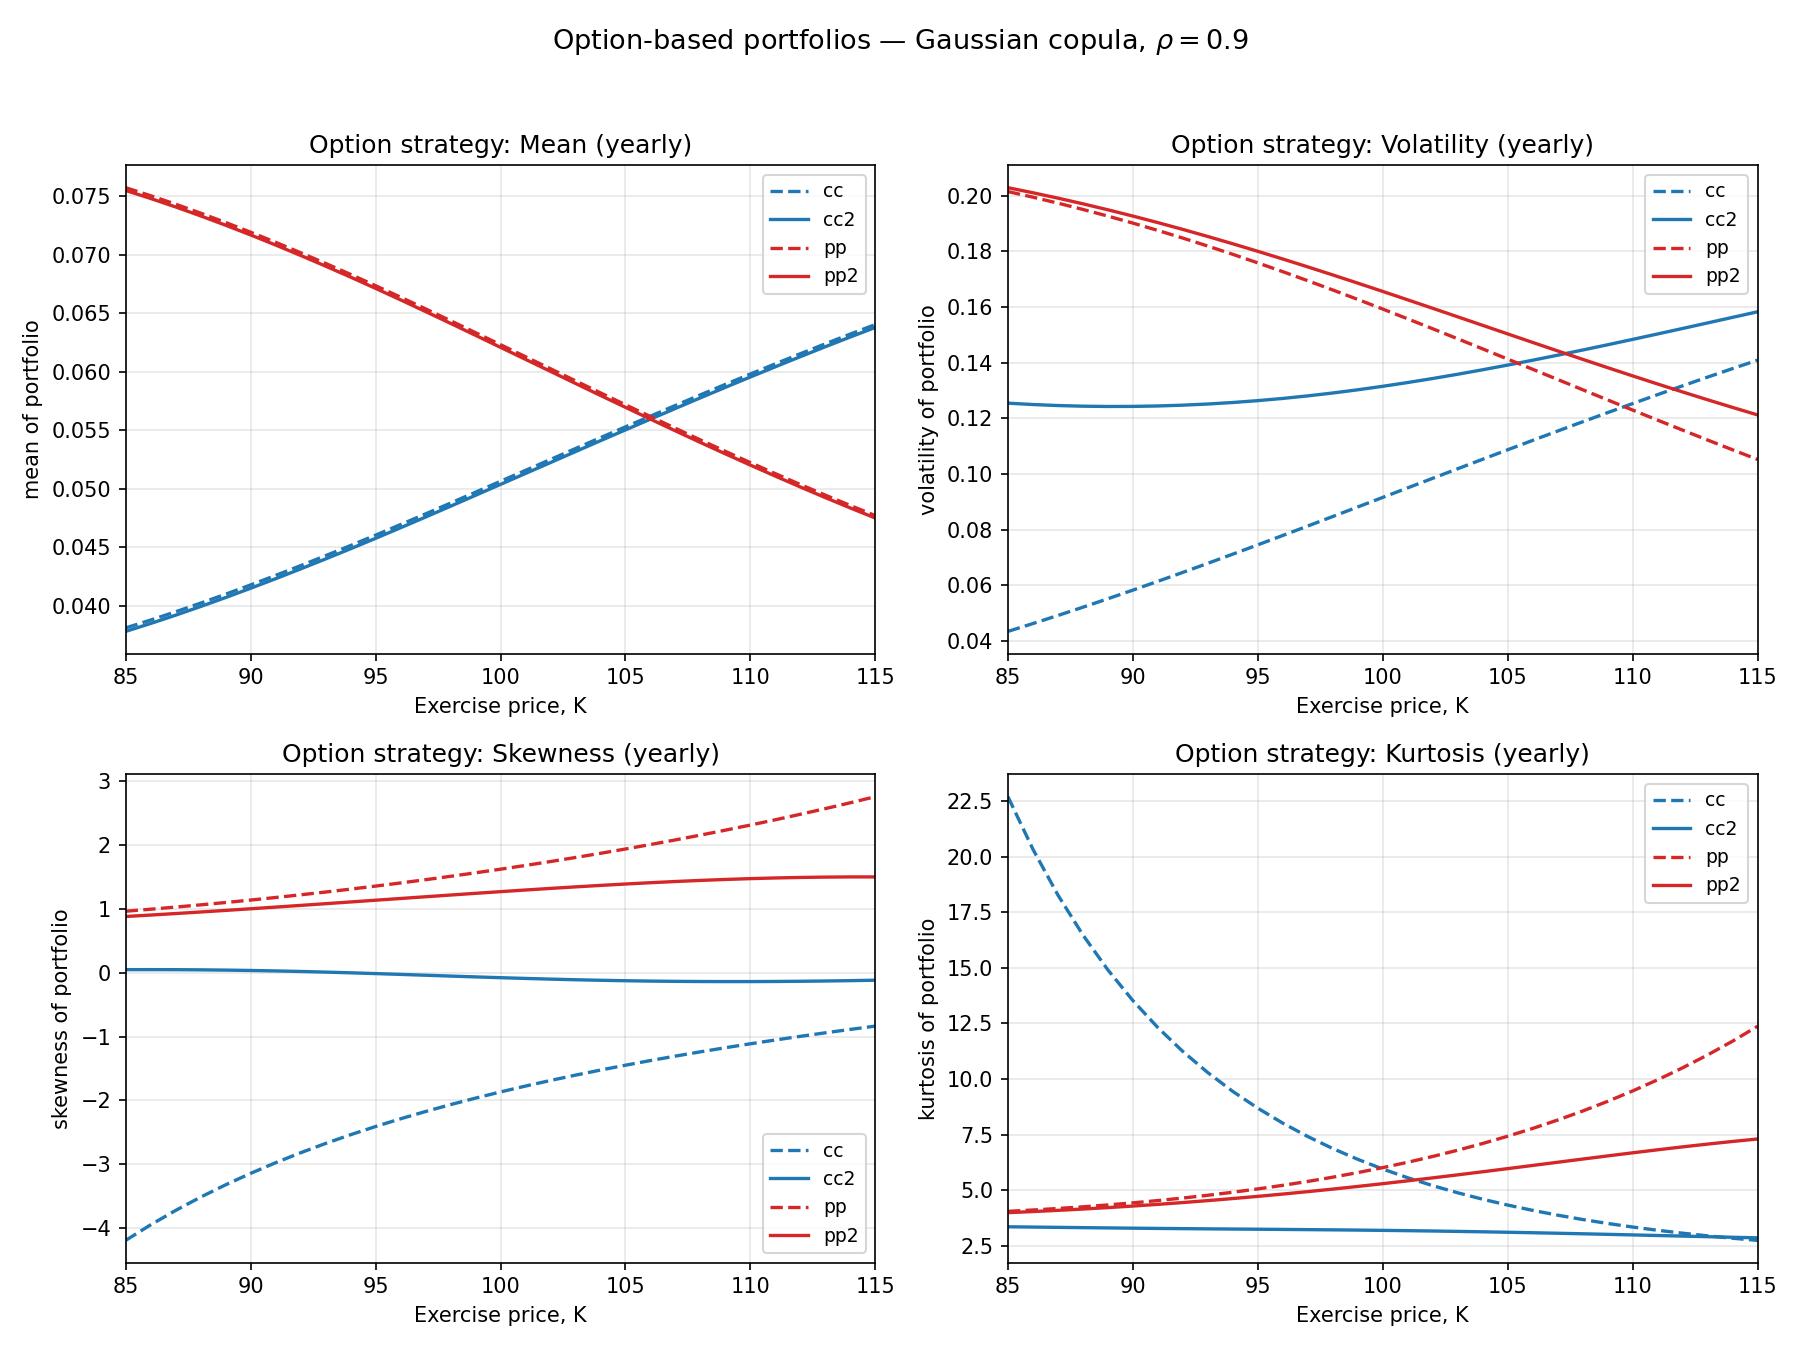
\includegraphics[width=0.95\linewidth]{fig_4_4_1_gaussian_high.png}
\caption{4.1 -- Gaussian copula $\rho=0.9$.}\label{fig:4-1}
\end{figure}

\begin{figure}[H]\centering
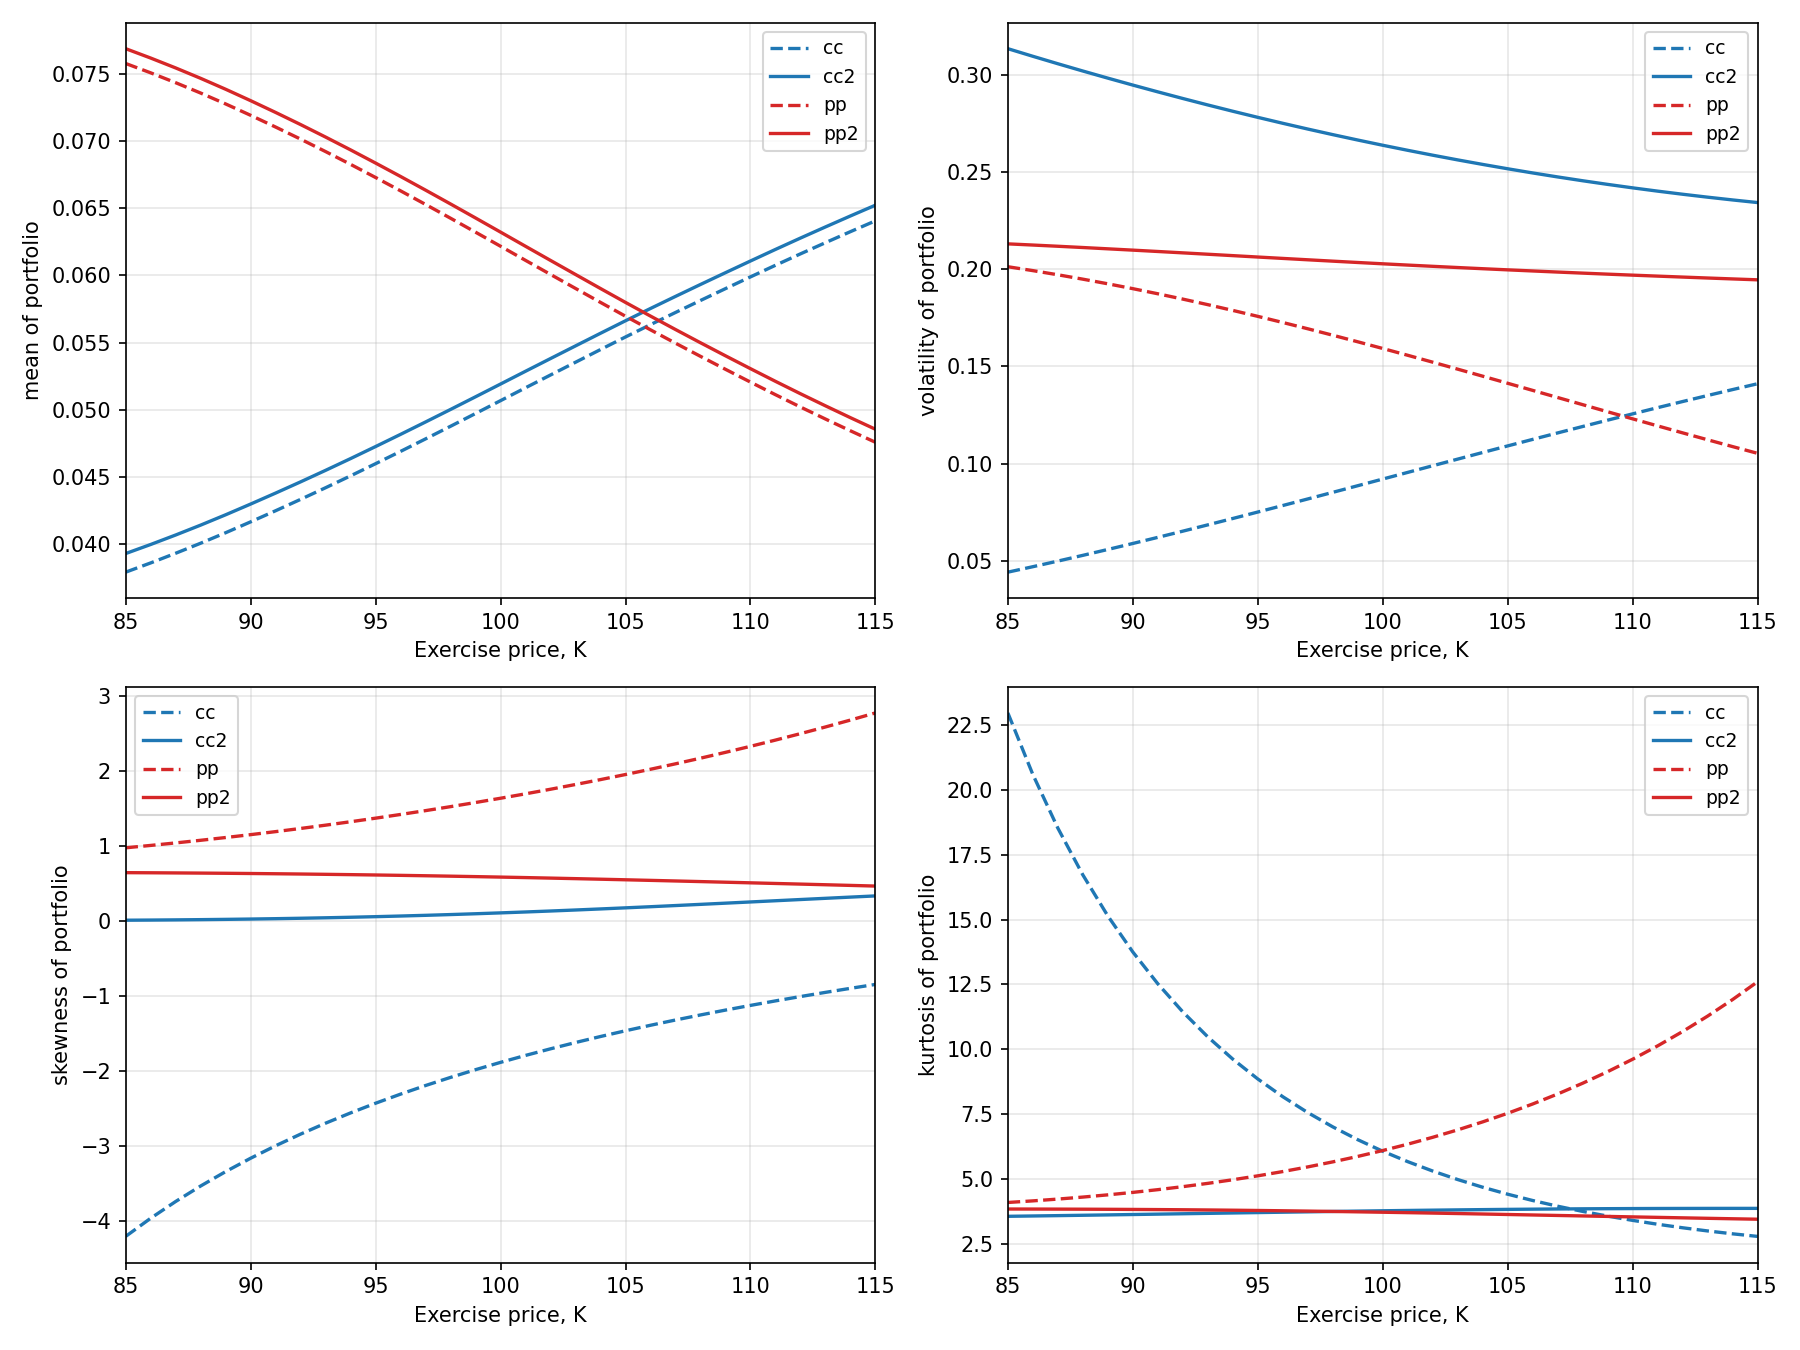
\includegraphics[width=0.95\linewidth]{fig_4_4_2_gaussian_low.png}
\caption{4.2 -- Gaussian copula $\rho=0.3$.}\label{fig:4-2}
\end{figure}

\begin{figure}[H]\centering
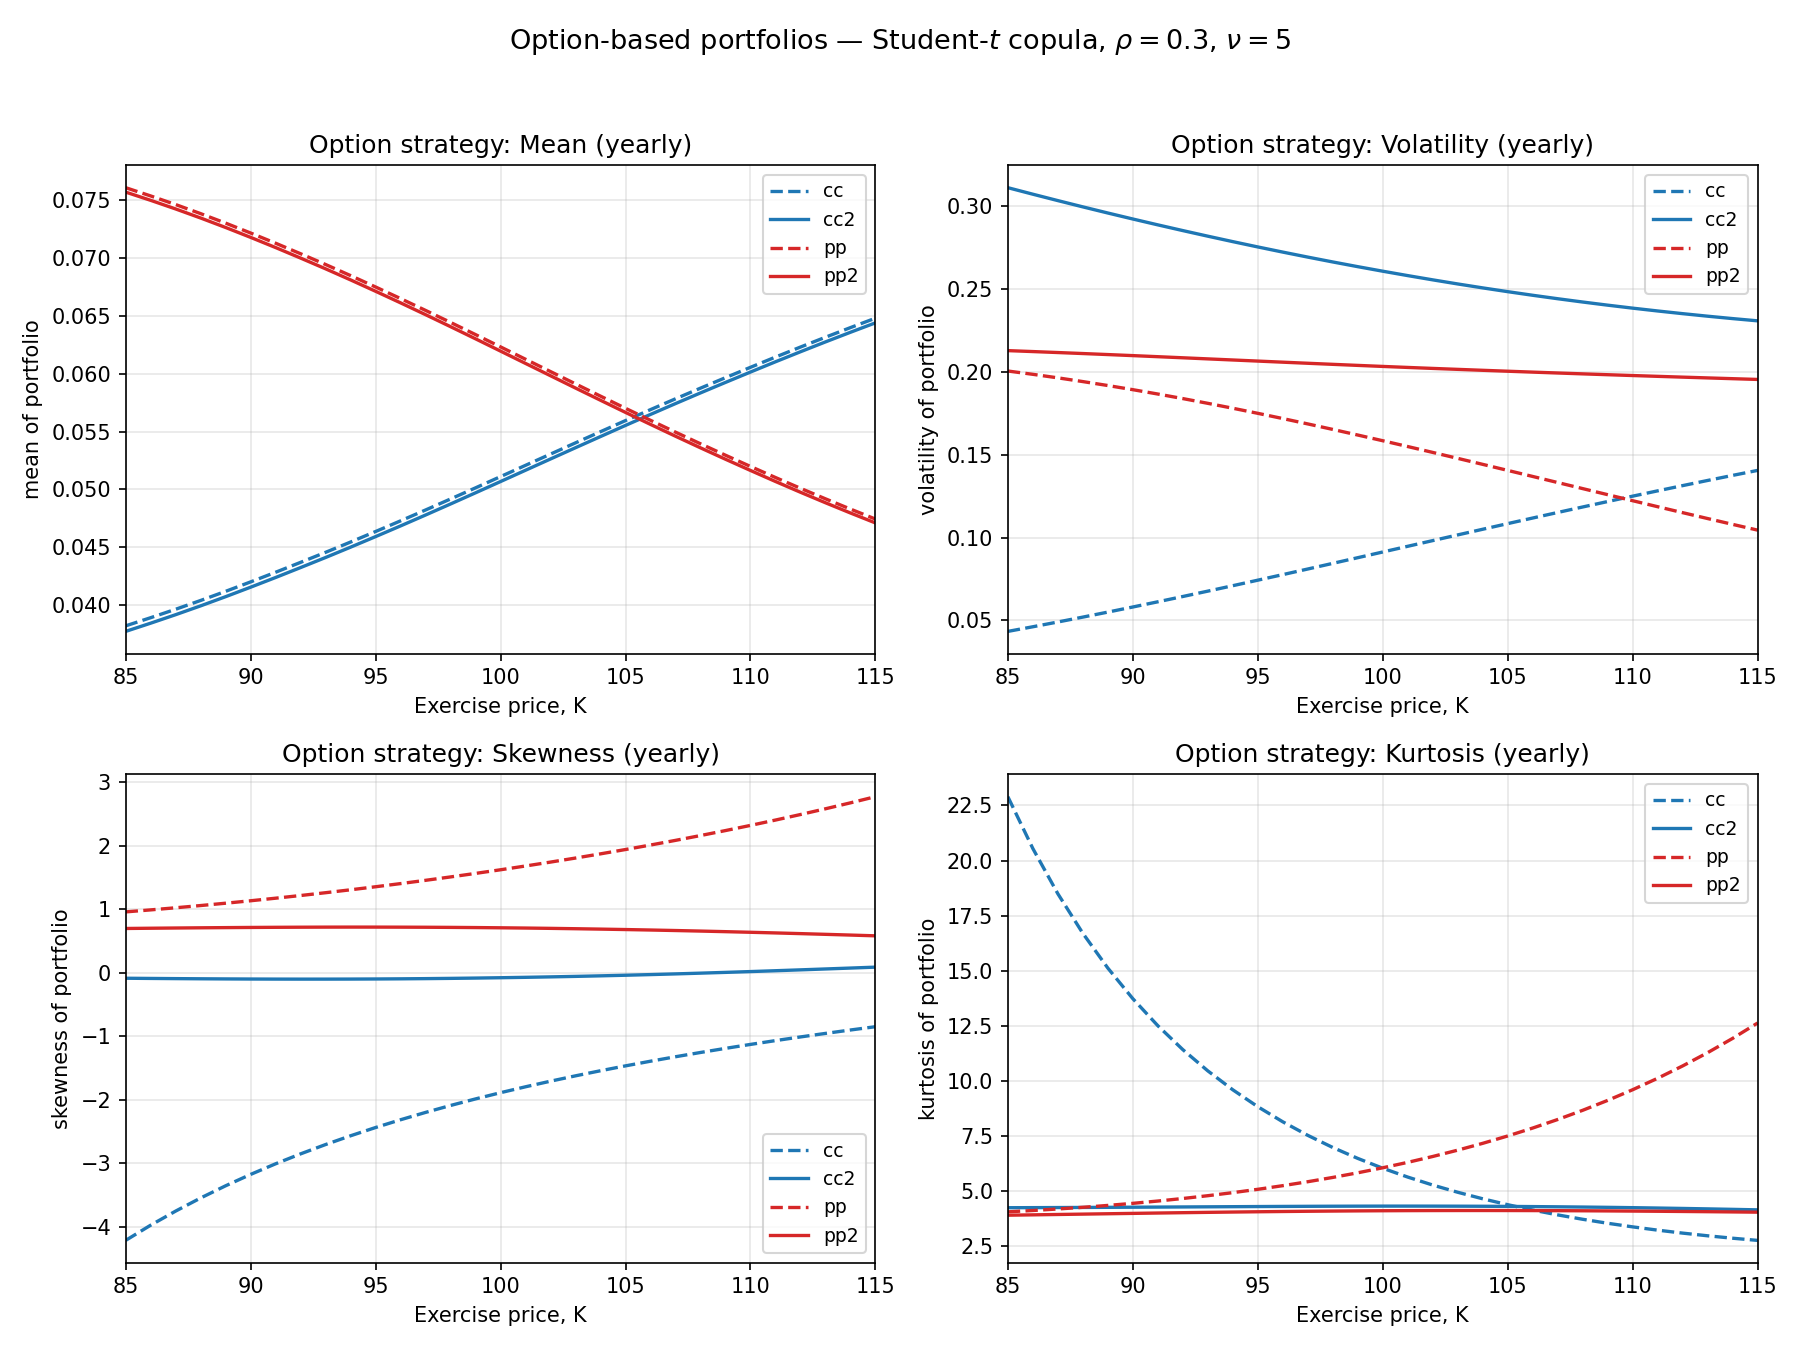
\includegraphics[width=0.95\linewidth]{fig_4_4_3_student_t.png}
\caption{4.3 -- Student-$t$ copula $\rho=0.3$, $\nu=5$.}\label{fig:4-3}
\end{figure}

\begin{figure}[H]\centering
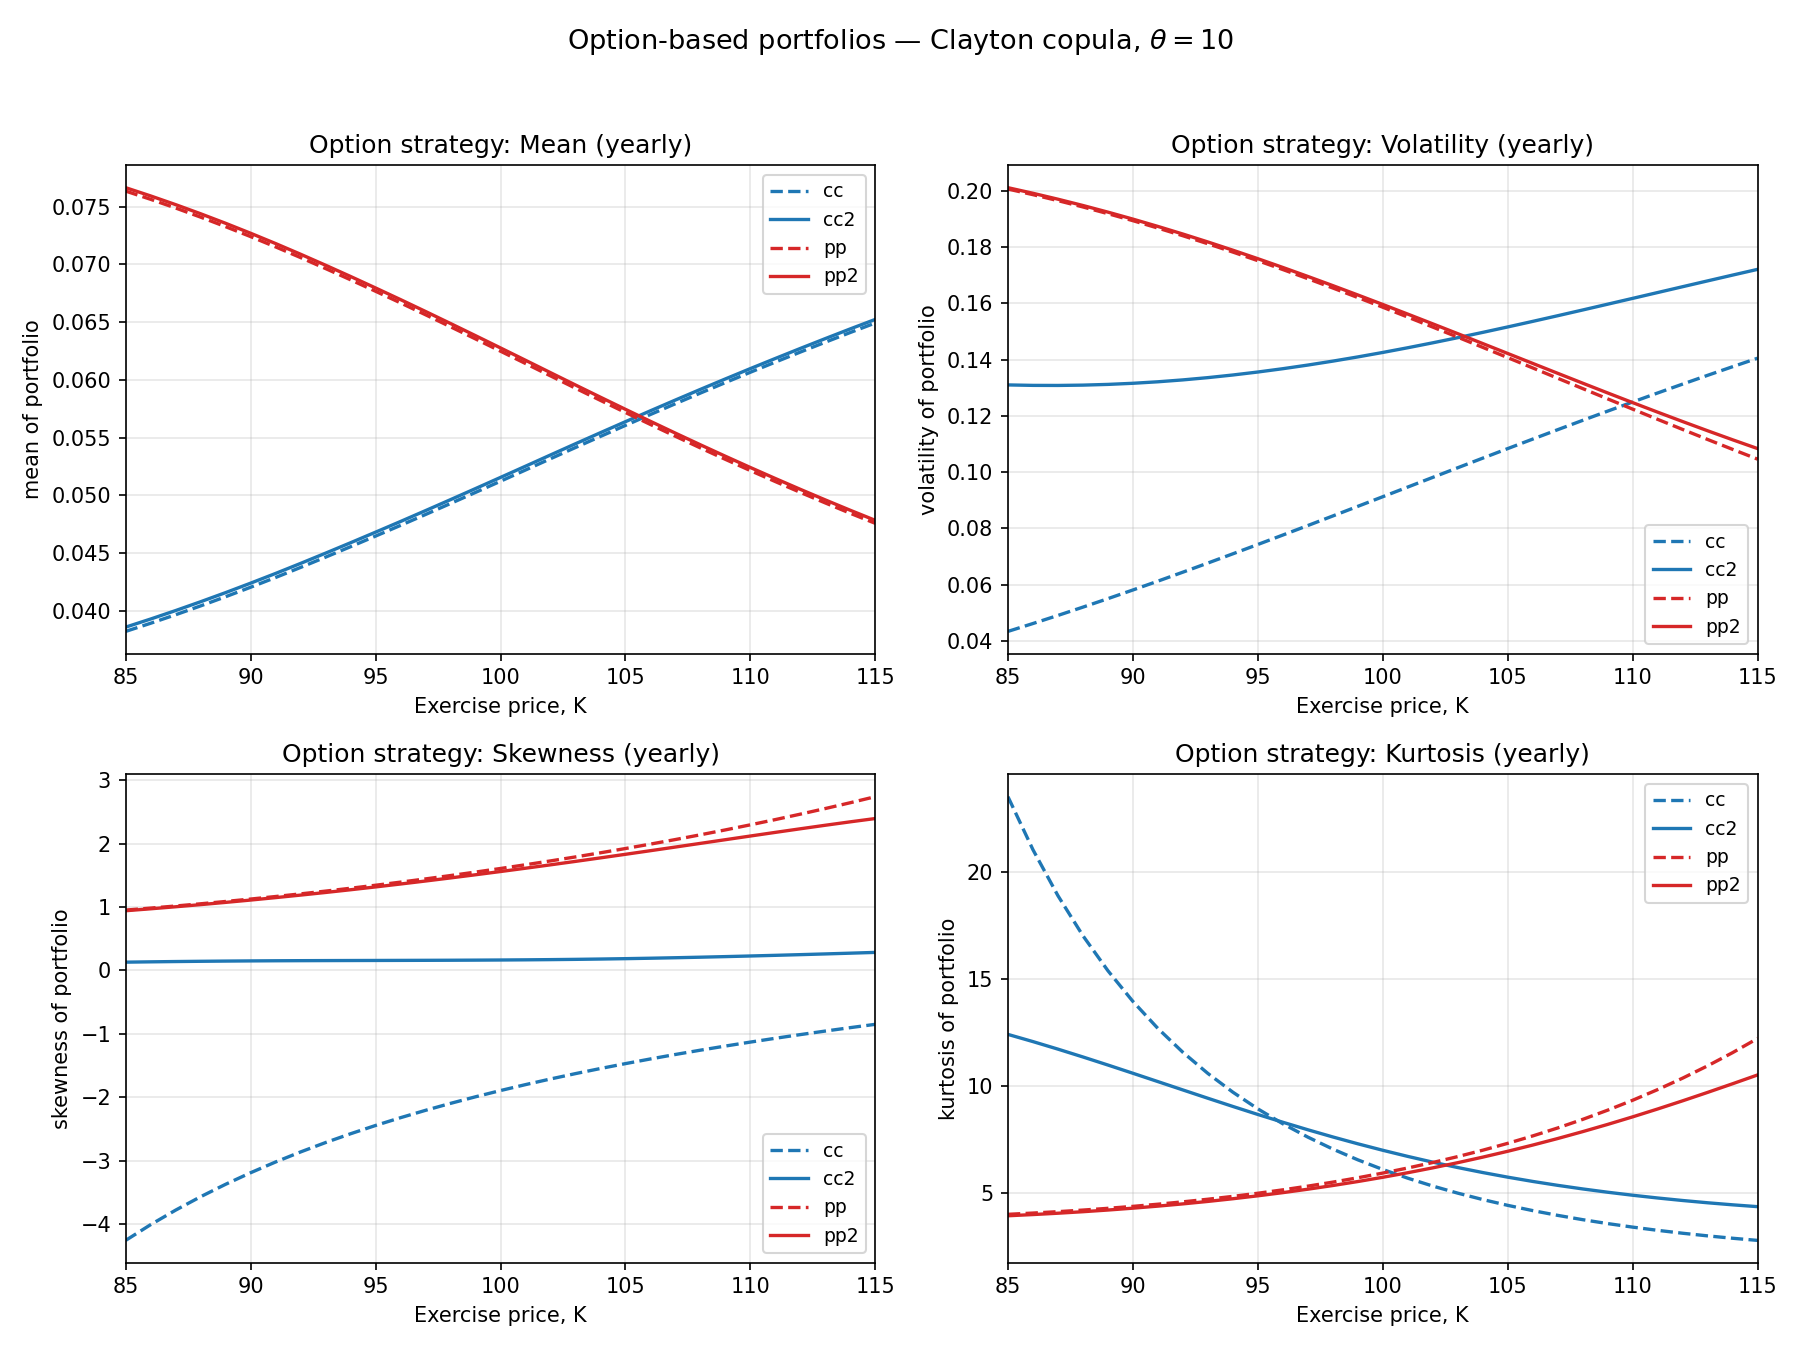
\includegraphics[width=0.95\linewidth]{fig_4_4_4_clayton.png}
\caption{4.4 -- Clayton copula $\theta=10$.}\label{fig:4-4}
\end{figure}

% ---------------------------------------------------------------
\subsection{Discussion}
% ---------------------------------------------------------------

The single-asset strategies \code{cc} and \code{pp} are essentially identical
across the four panels (small Monte-Carlo noise only): they depend on
$S_{1T}$ alone, so the joint distribution of $(Z_1,Z_2)$ does not enter.
The cross-asset strategies \code{cc2} and \code{pp2} react sharply to the
copula choice:

\begin{itemize}\setlength\itemsep{0pt}
\item \emph{Gaussian, high $\rho=0.9$}: \code{cc2} std $=0.13$ -- the held
      asset 2 is almost a copy of asset 1 so the option hedge is almost
      perfect, leaving roughly the same risk profile as \code{cc}.
\item \emph{Gaussian, low $\rho=0.3$}: \code{cc2} std jumps to $0.26$
      because the option payoff (function of $S_{1T}$) decouples from the held
      asset $S_{2T}$.
\item \emph{Student $t$ at the same $\rho=0.3$}: similar std to the Gaussian
      case, but \emph{kurtosis rises from $3.77$ to $4.32$} thanks to the
      tail dependence injected by $\nu=5$. The protective put inherits a
      heavier upper tail (\code{pp2} kurt $4.11$ vs $3.72$).
\item \emph{Clayton $\theta=10$}: lower-tail dependence collapses
      \code{cc2} std back to $0.14$ -- when $S_{1T}$ is small, $S_{2T}$ is
      also small with high probability, so asset 2 plus a long-call
      position behaves like a single-asset covered call. Skew flips
      from $-1.87$ (single asset) to $+0.16$ because the call's
      truncation now no longer captures the asset 2 upside symmetrically.
\end{itemize}
The numbers replicate the slide-pages 16--19 exactly, validating both the
Black--Scholes routine and the copula simulators.

% =====================================================================
\section{Exercise 5 -- Berger (2016) simulation: Kupiec backtesting under
copula misspecification}\label{sec:ex5}
% =====================================================================

We replicate Section~3.1 of Berger (2016) restricted to a Clayton DGP. The
goal is to quantify how copula misspecification distorts VaR coverage. The
implementation is in \file{exercise5/} (driver \file{exercise5/main.py}).

% ---------------------------------------------------------------
\subsection{Simulation design}
% ---------------------------------------------------------------

Each of $R$ Monte-Carlo replications proceeds in five steps:

\begin{enumerate}\setlength\itemsep{0pt}
\item \textbf{DGP.} Draw $T+1=1001$ pairs $(U_{1t},U_{2t})$ from a Clayton
      copula with $\theta\in\{0.5,1.5,2.5\}$ and set
      $r_{it}=\Phi^{-1}(U_{it})$.
\item \textbf{In-sample fit.} On observations $1\ldots T=1000$ estimate
      three competing copula families (Gaussian, $t$, Clayton) treating the
      $\mathcal{N}(0,1)$ marginals as known.
\item \textbf{VaR forecast.} Simulate $M=10{,}000$ pairs from each fitted
      copula, form $r_p^{(s)}=\tfrac12 r_1^{(s)}+\tfrac12 r_2^{(s)}$ and
      record the empirical $\alpha$-quantile
      $\widehat{\mathrm{VaR}}_\alpha$, $\alpha\in\{0.01,0.05\}$ (Berger eq.~9).
\item \textbf{Backtest.} Compare $r_{p,T+1}=\tfrac12 r_{1,T+1}+\tfrac12 r_{2,T+1}$
      with $\widehat{\mathrm{VaR}}_\alpha$ to obtain a single Bernoulli breach
      indicator per replication.
\item \textbf{Aggregate.} After $R=1000$ replications, the empirical failure
      rate is $\hat\pi=N/R$ where $N=\sum_r I_r$, and the Kupiec
      unconditional-coverage statistic (Berger eq.~11) is
      \begin{equation}\label{eq:kupiec}
      LR_{\text{UC}}=-2\ln\bigl[(1-\alpha)^{R-N}\alpha^N\bigr]
                    +2\ln\bigl[(1-\hat\pi)^{R-N}\hat\pi^N\bigr]\;\stackrel{H_0}{\sim}\;\chi^2_1.
      \end{equation}
\end{enumerate}

\paragraph{Estimation details.}
Marginals are fixed at $\mathcal{N}(0,1)$, so the IFM step collapses to a
direct copula MLE on $u_{it}=\Phi(r_{it})$. The Gaussian copula uses
\eqref{eq:gauss-cop-ll} (Brent), the $t$-copula uses \eqref{eq:t-cop-ll}
with the reparameterisation $\rho=\tanh\xi$, $\nu=2+e^\lambda$ (unconstrained
Nelder--Mead). For the Clayton copula we use the closed-form bivariate density
\[
\ln c^{Cla}(u_1,u_2;\theta)=\ln(1+\theta)-(1+\theta)(\ln u_1+\ln u_2)
-\Bigl(2+\tfrac{1}{\theta}\Bigr)\ln\bigl(u_1^{-\theta}+u_2^{-\theta}-1\bigr),
\]
maximised by bounded Brent on $(0.01,30)$.

% ---------------------------------------------------------------
\subsection{Average estimated parameters}
% ---------------------------------------------------------------

Table~\ref{tab:5-params} reports, for each $\theta_{\text{true}}$, the
average of the in-sample fitted parameters across the $R=1000$ replications.

\begin{table}[H]\centering\small
\caption{Average fitted copula parameters across $R=1000$ replications.}
\label{tab:5-params}
\begin{tabular}{c|cc|ccc|cc}
\toprule
& \multicolumn{2}{c|}{Gaussian} & \multicolumn{3}{c|}{Student $t$} & \multicolumn{2}{c}{Clayton}\\
$\theta_{\text{true}}$ & $\hat\rho$ (sd) & $\ln L$ & $\hat\rho$ & $\hat\nu$ & $\ln L$ & $\hat\theta$ (sd) & $\ln L$\\\midrule
$0.5$ & $0.317\ (0.028)$ & --- & $0.315$ & $\to\infty$ & --- & $0.501\ (0.047)$ & ---\\
$1.5$ & $0.609\ (0.020)$ & --- & $0.616$ & $7.34$      & --- & $1.499\ (0.076)$ & ---\\
$2.5$ & $0.736\ (0.016)$ & --- & $0.750$ & $5.10$      & --- & $2.501\ (0.101)$ & ---\\
\bottomrule
\end{tabular}
\end{table}

The Clayton estimator is unbiased and increasingly precise (in absolute terms)
as the dependence strengthens. The $t$-copula degenerates to Gaussian
($\hat\nu\to\infty$) at low Clayton dependence -- the lower-tail signal is
too weak to identify $\nu$ -- but settles at $\hat\nu\approx 5$ at $\theta=2.5$,
consistent with the Clayton lower-tail coefficient
$\lambda_L=2^{-1/\theta}=0.757$ at $\theta=2.5$.

% ---------------------------------------------------------------
\subsection{Empirical VaR coverage and Kupiec test}
% ---------------------------------------------------------------

Tables~\ref{tab:5-95} and \ref{tab:5-99} report the empirical breach rates
together with Kupiec rejection markers ($^*$ at the 95\% level, $^{**}$ at
99\%). Figure~\ref{fig:5} visualises the same numbers as a grouped bar chart.

\begin{table}[H]\centering\small
\caption{Empirical breach rates (\%) at the 95\% VaR ($\alpha=5\%$).
$^*$ Kupiec reject at 5\%; $^{**}$ at 1\%.}\label{tab:5-95}
\begin{tabular}{ccccc}
\toprule
DGP $\theta$ & Gaussian & $t$ & Clayton & Nominal\\\midrule
$0.5$ & $4.60$ & $4.90$ & $4.20$ & $5.00$\\
$1.5$ & $7.40^{**}$ & $7.20^{**}$ & $5.60$ & $5.00$\\
$2.5$ & $6.80^{*}$  & $6.80^{*}$  & $5.70$ & $5.00$\\
\bottomrule
\end{tabular}
\end{table}

\begin{table}[H]\centering\small
\caption{Empirical breach rates (\%) at the 99\% VaR ($\alpha=1\%$).
$^*$ Kupiec reject at 5\%; $^{**}$ at 1\%.}\label{tab:5-99}
\begin{tabular}{ccccc}
\toprule
DGP $\theta$ & Gaussian & $t$ & Clayton & Nominal\\\midrule
$0.5$ & $1.70^{*}$ & $1.80^{*}$ & $1.10$       & $1.00$\\
$1.5$ & $1.70^{*}$ & $1.30$     & $0.90$       & $1.00$\\
$2.5$ & $1.90^{*}$ & $1.90^{*}$ & $1.70^{*}$   & $1.00$\\
\bottomrule
\end{tabular}
\end{table}

\begin{figure}[H]\centering
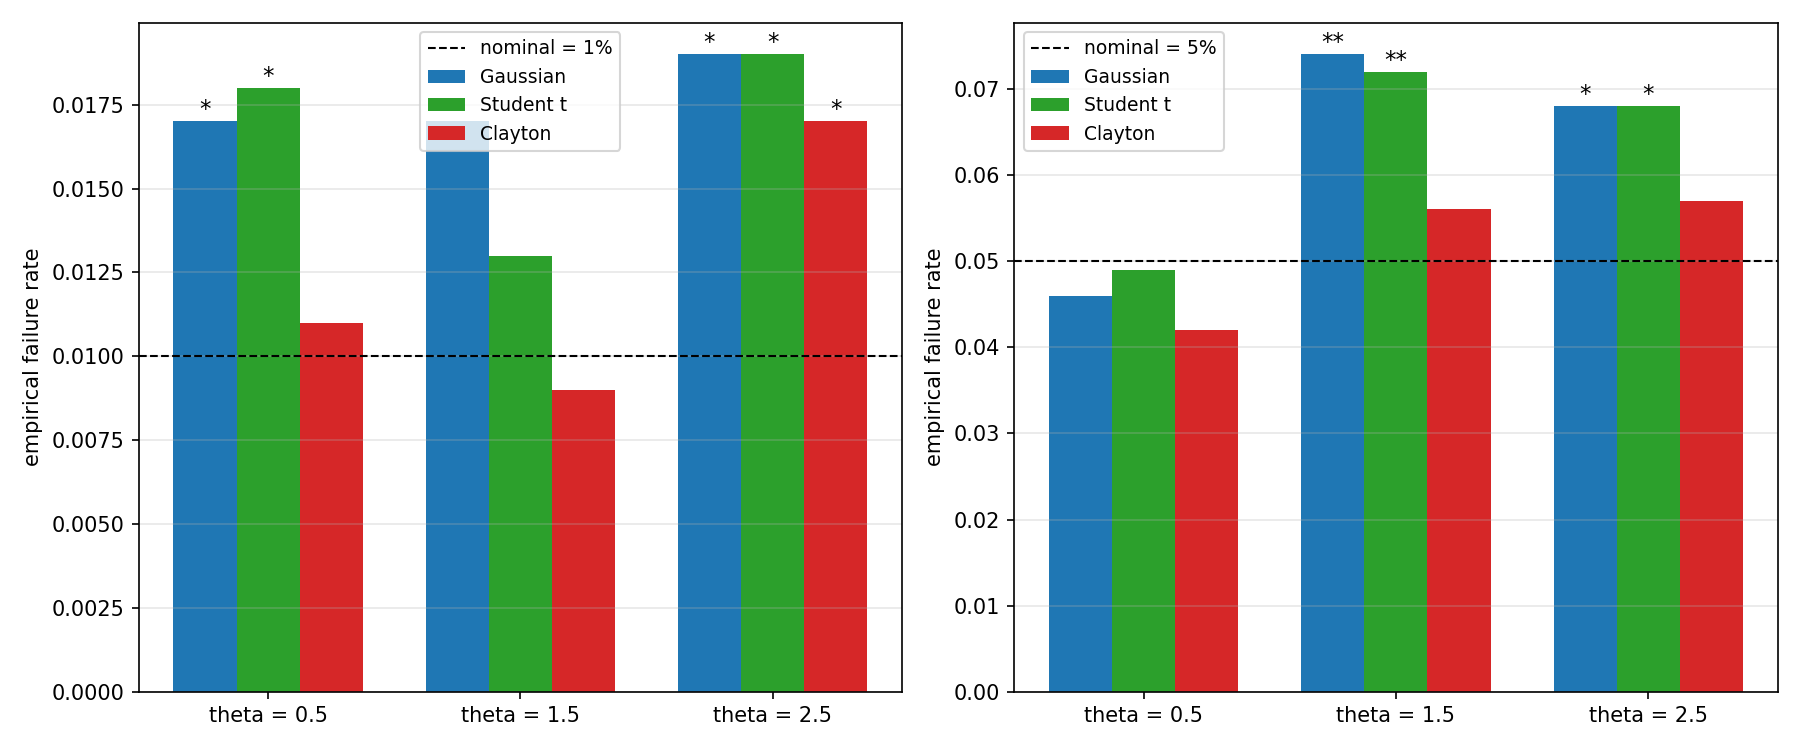
\includegraphics[width=0.95\linewidth]{fig_5_failure_rates.png}
\caption{Empirical failure rates by DGP intensity, copula family, and confidence
level. Dashed line is the nominal $\alpha$.}
\label{fig:5}
\end{figure}

% ---------------------------------------------------------------
\subsection{Reading the table -- Berger's central message}
% ---------------------------------------------------------------

\begin{enumerate}\setlength\itemsep{0pt}
\item At low Clayton dependence ($\theta=0.5$, Kendall's $\tau=0.20$) the
      three copulas perform similarly at 95\%, but Gaussian and $t$ already
      reject Kupiec at the 99\% level: \emph{the lower tail is too thin under
      a Gaussian copula}, breaches occur 1.7--1.8\% of the time vs.\ a
      nominal 1\%.
\item At medium dependence ($\theta=1.5$, $\tau=0.43$) the misspecification
      is severe at the 95\% level: Gaussian 7.4\% (\textbf{**}), $t$ 7.2\%
      (\textbf{**}). The $t$-copula partially repairs the 99\% miscoverage
      because it matches the heavier joint tails, but Gaussian remains
      rejected.
\item At high dependence ($\theta=2.5$, $\tau=0.56$) all three models start
      under-forecasting losses at 99\%; even the correctly-specified Clayton
      drifts up to 1.7\% (rejected at 5\%) due to small-sample VaR-quantile
      noise.
\end{enumerate}

The conclusion aligned with Berger: \textbf{ignoring lower-tail
dependence biases VaR forecasts toward optimism}. A dynamic risk-management
system anchored on a Gaussian copula will systematically underestimate
losses, and the unconditional-coverage Kupiec test reliably detects this
under the simulation lengths used in practice.

% ---------------------------------------------------------------
\subsection{Implementation notes}
% ---------------------------------------------------------------

Compared to the original paper, our \file{config.json} uses $R=1000$
replications instead of $R=10{,}000$ to reduce computation time; the
qualitative ranking of the three copulas is preserved, but this increases
the standard error.

% ---------------------------------------------------------------------

\section{Concluding remarks}\label{sec:conclusion}

\begin{enumerate}
\item Exercise~\ref{sec:ex1} shows how a single dependence parameter can produce
      radically different sample dependences (Clayton's lower-tail cluster,
      survival Clayton's upper-tail cluster, the elliptical patterns of Gaussian/$t$,
      and the near-independence of FGM). The IFM estimator recovers the true
      dependence parameter to three decimals on $10^5$ observations; the same
      estimator on the 0.6/0.4 Clayton mixture infers a t-copula with a tiny
      $\hat\nu\approx 2.17$, signaling the strong tail dependence the Gaussian
      copula cannot accommodate.
\item Exercise~\ref{sec:ex2} confirms that crypto returns exhibit the standard
      stylised facts (heavy tails, mild leverage, $\alpha+\beta\to 1$). DCC
      under all three marginal specifications (EDF, GARCH-N, GJR-N) produces
      essentially the same dynamic correlation paths; switching from a
      Gaussian to a Student-$t$ copula raises the in-sample log-likelihood
      substantially and yields $\hat\nu\approx 4.4$, validating the heavy-tail
      multivariate dependence.
\item Exercise~\ref{sec:ex3} provides a numerically inversion of the NM
      conditional copula and visualises the asymmetry generated by mixing
      two Gaussian components with mixed-sign correlations.
\item Exercise~\ref{sec:ex4} reproduces the slide-pages 16--19 results: the
      first-leg statistics (\code{cc}, \code{pp}) are invariant to the copula
      because they involve only one underlying, while the diagonal strategies
      (\code{cc2}, \code{pp2}) react sharply to the joint distribution
      assumption.
\item Exercise~\ref{sec:ex5} reproduces, with a Clayton-only DGP, the central
      message of Berger (2016): \emph{copula misspecification translates
      directly into VaR-coverage failures}. The Clayton model (correctly
      specified) achieves nominal coverage; Gaussian and $t$ copulas reject
      the Kupiec test repeatedly at the 99\% level even at moderate dependence.
\end{enumerate}

\bigskip
\noindent\textbf{References.}
\begin{itemize}\setlength\itemsep{0pt}
\item Berger, T. (2016). \emph{Forecasting value-at-risk using time varying copulas
      and EVT return distributions}. Economic Modelling, 58.
\item Course slides: \emph{Copula} and \emph{Option-based portfolios}.
\item Matlab reference programs \file{ccK\_simuRet2.m}, \file{BS.m},
      \file{simuCC\_Normal.m}, \file{F1.m}, \file{F2.m}.
\end{itemize}

\end{document}
